% -*- coding: utf-8 -*-
\documentclass[10pt,journal,twocolumn]{IEEEtran}
\usepackage[utf8]{inputenc}
\usepackage{fontspec}
\usepackage{xeCJK}
\setCJKmainfont{SimSun}[BoldFont=SimHei, ItalicFont=KaiTi]
\setCJKsansfont{SimHei}
\setCJKmonofont{FangSong}

\usepackage{amsmath,amssymb,amsfonts}
\usepackage{graphicx}
\usepackage{booktabs}
\usepackage{multirow}
\usepackage{enumitem}
\usepackage{hyperref}
\usepackage{xcolor}
\usepackage{caption}
\usepackage{subcaption}
\usepackage{algorithm}
\usepackage{algorithmic}
\usepackage{cite}
\usepackage{url}

\hypersetup{colorlinks=true, linkcolor=blue, citecolor=blue, urlcolor=blue}
\graphicspath{{../figures/}}

\newcommand{\cmark}{\textcolor{green!60!black}{$\checkmark$}}
\newcommand{\xmark}{\textcolor{red}{$\times$}}
\newcommand{\E}{\mathbb{E}}

\title{大语言模型训练中强化学习算法的综合综述：\\PPO、DPO、GRPO与DAPO}

\author{
\IEEEauthorblockN{Aitachi}
\IEEEauthorblockA{\texttt{44158892@qq.com}}
}

\date{2025}

\begin{document}
\maketitle

% 中文版 Section 1: 引言
\begin{abstract}
强化学习（RL）已成为对齐和增强大语言模型（LLM）的核心技术。本综述对四种主流RL算法进行了全面系统的分析：近端策略优化（PPO）、直接偏好优化（DPO）、组相对策略优化（GRPO）和动态优势策略优化（DAPO。我们为每个算法提供了严格的数学公式推导，比较了其架构设计和计算需求，并在数学推理基准（包括AIME 2024）上评估了其实证性能。分析揭示了从基于价值的方法（PPO）到基于分组的方法（GRPO/DAPO）的清晰演进轨迹。具体而言，DAPO通过三大创新——非对称Clip-Higher、动态采样和Token级损失归一化——在AIME 2024上达到50\%的准确率，较朴素GRPO实现67\%的相对提升。我们提供了实用的算法选择指南，并指出了未来研究的开放性挑战。据我们所知，这是首个在统一数学框架下对这四种算法进行并排实验评估的综述。
\end{abstract}

\begin{IEEEkeywords}
强化学习，大语言模型，PPO，DPO，GRPO，DAPO，RLHF，对齐，数学推理
\end{IEEEkeywords}

%=============================================================
\section{引言}
\label{sec:intro}

以GPT-4~\cite{achiam2023gpt4}、LLaMA~\cite{touvron2023llama}和Qwen2.5~\cite{yang2024qwen25}为代表的大语言模型（LLM）从根本上改变了自然语言处理领域，在数学推理、代码生成、科学分析和创意写作等方面展现了前所未有的能力。然而，仅通过大规模语料库上的下一词元预测训练的模型，其输出往往在有用性、安全性和事实准确性方面与人类偏好不一致。

基于人类反馈的强化学习（RLHF）~\cite{christo2017deep, ouyang2022instructgpt}已成为弥合这一对齐差距的主流范式。标准RLHF流程包含三个阶段：（1）在高质示范数据上进行监督微调（SFT）；（2）基于人类偏好比较训练奖励模型（RM）；（3）使用训练好的奖励模型进行基于RL的策略优化。虽然阶段1和2相对标准化，但阶段3中RL算法的选择对训练稳定性、计算效率和最终模型性能具有深远影响。

LLM训练中RL算法的演进正在急剧加速：

\begin{itemize}[leftmargin=*, itemsep=2pt]
\item \textbf{PPO}~\cite{schulman2017ppo}（2017年）：基础性算法，需要策略网络（Actor）和价值网络（Critic）双网络架构。它是InstructGPT~\cite{ouyang2022instructgpt}和ChatGPT背后的核心算法，但双网络架构需要大量GPU内存。
\item \textbf{DPO}~\cite{rafailov2023dpo}（2023年）：范式转变，通过从偏好对推导闭式损失函数消除了显式奖励建模。DPO简化了训练流程，但需要预先收集的偏好数据。
\item \textbf{GRPO}~\cite{deepseek2025r1, shao2024deepseekmath}（2025年）：由DeepSeek团队提出，通过使用组级奖励统计作为优势基线消除了价值网络，GPU内存减少约50\%。
\item \textbf{DAPO}~\cite{yu2025dapo}（2025年）：由字节跳动提出，通过三大创新扩展GRPO——非对称Clip-Higher、动态采样和Token级损失，在AIME 2024上达到50\%的准确率。
\end{itemize}

本综述的贡献如下：
\begin{enumerate}[leftmargin=*, itemsep=1pt]
\item 统一的数学框架，四种算法使用一致的符号表示，可直接进行跨算法目标函数和设计选择的比较。
\item 系统的架构比较，涵盖网络需求、裁剪策略、损失粒度和KL约束机制。
\item 在数学推理基准上的实验评估，包含训练效率、模型质量和资源利用的量化结果。
\item 基于任务特征和资源约束的实用算法选择指南。
\end{enumerate}

本文其余部分组织如下：第\ref{sec:bg}节建立背景和符号；第\ref{sec:ppo}--\ref{sec:dapo}节详细介绍每个算法；第\ref{sec:compare}节进行比较分析；第\ref{sec:exp}节展示实验结果；第\ref{sec:discuss}节讨论影响和未来方向；第\ref{sec:conclusion}节为结论。

% 中文版 Section 2: 背景与预备知识
\section{背景与预备知识}
\label{sec:bg}

\subsection{LLM中的强化学习建模}

在LLM对齐的语境下，训练过程被建模为上下文赌博机（Contextual Bandit）问题而非完整的马尔可夫决策过程（MDP）。这种建模是合理的，因为模型在自回归地生成完整响应后才接收奖励信号。形式化定义如下：

\begin{itemize}[leftmargin=*, itemsep=1pt]
\item \textbf{状态/上下文} $x \sim \mathcal{D}$：从训练分布$\mathcal{D}$中采样的输入提示词。
\item \textbf{动作/响应} $y = (y_1, y_2, \ldots, y_T)$：模型生成的词元序列，$T$为响应长度。
\item \textbf{策略} $\pi_\theta(y|x) = \prod_{t=1}^{T} \pi_\theta(y_t | x, y_{<t})$：以$\theta$为参数的自回归语言模型。
\item \textbf{奖励} $r(x, y) \in \mathbb{R}$：评估给定提示词$x$下响应$y$质量的标量信号。
\end{itemize}

优化目标是寻找使期望奖励最大化的策略参数$\theta^*$：
\begin{equation}
\theta^* = \arg\max_\theta J(\theta) = \arg\max_\theta \E_{x \sim \mathcal{D},\ y \sim \pi_\theta(\cdot|x)}\left[r(x, y)\right]
\label{eq:obj}
\end{equation}

一个关键挑战是防止策略偏离参考模型$\pi_{\text{ref}}$（通常是SFT检查点）过远，因为无约束优化可能导致奖励黑客攻击和模式坍塌。不同算法通过不同机制解决这一约束：显式KL惩罚（GRPO）、隐式正则化（DPO）、裁剪代理目标（PPO、DAPO）或其组合。

\subsection{RLHF流程详解}

标准RLHF流程包含三个阶段：

\textbf{阶段1 --- 监督微调（SFT）：}在高质量示范数据$\{(x_i, y_i^*)\}_{i=1}^{N}$上使用最大似然估计微调预训练语言模型：
\begin{equation}
\mathcal{L}_{\text{SFT}}(\theta) = -\E_{(x,y^*) \sim \mathcal{D}_{\text{demo}}}\left[\log \pi_\theta(y^*|x)\right]
\end{equation}
得到的模型$\pi_{\text{SFT}}$作为后续RL训练的初始化和参考模型$\pi_{\text{ref}}$。

\textbf{阶段2 --- 奖励模型训练：}在人类偏好对$(x, y_w, y_l)$上训练奖励模型$r_\phi(x, y)$，其中$y_w \succ y_l$表示$y_w$优于$y_l$。Bradley-Terry模型提供训练目标：
\begin{equation}
\mathcal{L}_{\text{RM}}(\phi) = -\E\left[\log \sigma\left(r_\phi(x, y_w) - r_\phi(x, y_l)\right)\right]
\end{equation}
其中$\sigma(\cdot)$为Logistic Sigmoid函数。

\textbf{阶段3 --- RL策略优化：}使用RL算法对语言模型策略$\pi_\theta$进行优化。这是算法选择（PPO、GRPO、DAPO）最关键的阶段。DPO通过直接在偏好对上优化完全绕过了阶段2和3。

\subsection{统一符号}

表\ref{tab:notation}建立了全文使用的统一符号体系。

\begin{table}[ht]
\centering
\caption{本文使用的统一数学符号}
\label{tab:notation}
\begin{tabular}{cl}
\toprule
\textbf{符号} & \textbf{定义} \\
\midrule
$\pi_\theta$ & 当前策略网络（正在训练的LLM） \\
$\pi_{\text{ref}}$ & 参考（冻结）策略，通常为SFT模型 \\
$\pi_{\theta_{\text{old}}}$ & 上一步更新的策略参数 \\
$r(x,y)$ & 奖励函数（学习型或规则型） \\
$\hat{A}$ & 优势函数估计值 \\
$r_t(\theta)$ & 重要性采样比率 $\pi_\theta/\pi_{\theta_{\text{old}}}$ \\
$\varepsilon$ & PPO/GRPO对称裁剪参数 \\
$\varepsilon_{\text{low}}, \varepsilon_{\text{high}}$ & DAPO非对称裁剪边界 \\
$\beta$ & KL惩罚系数或DPO温度 \\
$G$ & GRPO/DAPO的组采样大小 \\
$\gamma, \lambda$ & 折扣因子和GAE衰减参数 \\
$V_\phi$ & PPO的价值网络（Critic） \\
$y_w, y_l$ & 偏好对中的优选和拒绝响应 \\
$|o_i|$ & 第$i$个响应的词元长度 \\
\bottomrule
\end{tabular}
\end{table}

% 中文版 Section 3: PPO
\section{近端策略优化（PPO）}
\label{sec:ppo}

\subsection{算法概述与动机}

PPO~\cite{schulman2017ppo}由Schulman等人于2017年提出，至今仍是LLM对齐中应用最广泛的RL算法。它是InstructGPT~\cite{ouyang2022instructgpt}和早期ChatGPT版本的核心算法。PPO在策略梯度框架基础上引入裁剪代理目标，将策略更新约束在信赖域内，在保持样本效率的同时防止破坏性的大幅更新。

PPO的核心思想在于：原始策略梯度方法存在高方差和更新不稳定的问题。信赖域策略优化（TRPO）通过硬KL约束解决了这一问题，但其二阶优化的计算代价高昂。PPO通过裁剪概率比率，用一阶优化实现了类似的稳定性。

\subsection{裁剪代理目标}

PPO的核心是裁剪代理函数。设$r_t(\theta) = \frac{\pi_\theta(a_t|s_t)}{\pi_{\theta_{\text{old}}}(a_t|s_t)}$表示当前策略与旧策略的概率比率。裁剪目标为：
\begin{equation}
L^{\text{CLIP}}(\theta) = \E_t\!\left[\min\!\left(r_t(\theta)\hat{A}_t,\ \text{clip}(r_t(\theta), 1{-}\varepsilon, 1{+}\varepsilon)\hat{A}_t\right)\right]
\label{eq:ppo_clip}
\end{equation}
其中$\varepsilon$为超参数（通常取0.2），控制裁剪范围。

\textbf{直观解释：}当优势$\hat{A}_t > 0$（动作优于预期）时，目标鼓励增大$r_t$但在$1 + \varepsilon$处裁剪，防止策略更新过大。当$\hat{A}_t < 0$时，抑制该动作但在$1 - \varepsilon$处裁剪。这创建了目标函数中的一个``平坦''区域，为防止灾难性的大幅更新提供了鲁棒性。

\subsection{价值函数与熵奖励}

PPO维护一个独立的价值网络$V_\phi(s)$来估计期望回报。价值函数损失使用均方误差目标：
\begin{equation}
L^{VF}(\phi) = \E_t\left[\left(V_\phi(s_t) - \hat{V}_t^{\text{targ}}\right)^2\right]
\end{equation}

为鼓励探索和防止过早收敛到确定性策略，PPO添加熵奖励：
\begin{equation}
S[\pi_\theta](s_t) = -\sum_{a} \pi_\theta(a|s_t)\log\pi_\theta(a|s_t)
\end{equation}

\subsection{组合PPO目标}

完整的PPO目标结合了三个组件：
\begin{equation}
\boxed{L^{\text{PPO}}(\theta, \phi) = \E_t\left[L^{\text{CLIP}}(\theta) - c_1 L^{VF}(\phi) + c_2 S[\pi_\theta]\right]}
\label{eq:ppo}
\end{equation}
其中$c_1 = 0.5$和$c_2 = 0.01$为典型系数值。期望对当前策略收集的一批轨迹取平均。

\subsection{广义优势估计（GAE）}

优势函数$\hat{A}_t$使用GAE~\cite{schulman2016gae}进行估计，通过参数$\lambda$控制偏差-方差权衡：
\begin{equation}
\hat{A}_t^{\text{GAE}} = \sum_{l=0}^{\infty}(\gamma\lambda)^l\delta_{t+l}^{V}
\end{equation}
其中$\delta_t^{V} = r_t + \gamma V_\phi(s_{t+1}) - V_\phi(s_t)$为时序差分（TD）误差。当$\lambda = 0$时，GAE退化为单步TD误差（低方差、高偏差）；当$\lambda = 1$时，退化为蒙特卡洛回报（低偏差、高方差）。

\subsection{架构需求}

PPO需要\textbf{四个模型组件}同时加载到GPU内存中：
\begin{enumerate}[leftmargin=*, itemsep=1pt]
\item \textbf{Actor}（策略$\pi_\theta$）：正在训练的LLM。
\item \textbf{Critic}（价值$V_\phi$）：与Actor规模相当的独立网络。
\item \textbf{参考模型}（$\pi_{\text{ref}}$）：冻结副本，用于KL计算（RLHF中常见）。
\item \textbf{奖励模型}（$r_\psi$）：训练好的奖励函数。
\end{enumerate}

这使得PPO成为内存需求最高的算法，约为单LLM前向传播的$4\times$。对于70亿参数模型，通常需要4--8块A100 GPU配合模型并行。

\subsection{优势与局限}

\textbf{优势：}收敛性质已被充分研究；对超参数选择鲁棒；兼容任意奖励函数；具有策略梯度理论的坚实理论基础。

\textbf{局限：}价值网络带来高内存开销；奖励信号稀疏或含噪时训练不稳定；需要仔细的奖励模型训练；价值网络增加了显著的工程复杂度。

% 中文版 Section 4: DPO与GRPO
\section{直接偏好优化（DPO）}
\label{sec:dpo}

\subsection{动机：简化RLHF流程}

DPO~\cite{rafailov2023dpo}由Rafailov等人于2023年提出，代表了LLM对齐中的范式转变。DPO无需训练显式奖励模型再通过RL优化，而是推导出一个闭式损失函数，直接从偏好数据优化策略。其核心理论洞见在于：最优RLHF策略具有闭式解。

\subsection{从KL约束的RLHF目标推导}

KL约束的RLHF优化问题为：
\begin{equation}
\max_\pi \E_{x \sim \mathcal{D}, y \sim \pi}\left[r(x,y)\right] - \beta \cdot D_{\text{KL}}\!\left[\pi(\cdot|x) \| \pi_{\text{ref}}(\cdot|x)\right]
\end{equation}

闭式最优策略为：
\begin{equation}
\pi^*(y|x) = \frac{1}{Z(x)}\pi_{\text{ref}}(y|x)\exp\!\left(\frac{1}{\beta}r(x,y)\right)
\end{equation}
其中$Z(x) = \sum_y \pi_{\text{ref}}(y|x)\exp(r(x,y)/\beta)$为配分函数（计算不可行但在损失中会消去）。

\subsection{DPO损失函数}

将最优策略代入Bradley-Terry偏好模型并整理后，得到仅依赖策略和参考模型的DPO损失：
\begin{equation}
\boxed{
\begin{aligned}
L^{\text{DPO}}(\theta) &= -\E_{(x,y_w,y_l)}\bigl[\log\sigma\bigl(\beta\cdot h(y_w,y_l,x)\bigr)\bigr] \\
h(y_w,y_l,x) &= \log\frac{\pi_\theta(y_w|x)}{\pi_{\text{ref}}(y_w|x)} - \log\frac{\pi_\theta(y_l|x)}{\pi_{\text{ref}}(y_l|x)}
\end{aligned}
}
\label{eq:dpo}
\end{equation}

\textbf{解释：}$\sigma(\cdot)$内部的项是优选响应与拒绝响应的对数比率之差。DPO使$y_w$相对于$\pi_{\text{ref}}$的似然提升大于$y_l$的提升。温度$\beta$控制模型区分偏好和拒绝输出的锐度。

从训练好的策略中恢复的隐式奖励为：
\begin{equation}
\hat{r}(x,y) = \beta\log\frac{\pi_\theta(y|x)}{\pi_{\text{ref}}(y|x)}
\end{equation}

\subsection{架构需求}

DPO仅需\textbf{两个模型组件}：可训练策略$\pi_\theta$和冻结参考$\pi_{\text{ref}}$。无需奖励模型或价值网络，显著简化了训练流程。内存需求约为PPO的一半。

\subsection{优势与局限}

\textbf{优势：}四种算法中实现最简单；无需奖励模型训练；训练动态稳定；兼容离线偏好数据。

\textbf{局限：}需要预先收集的偏好对$(y_w, y_l)$，获取成本高；无法利用在线探索；性能受限于偏好数据的质量和覆盖范围；不适用于具有客观奖励信号的任务（如数学验证）。

%=============================================================
\section{组相对策略优化（GRPO）}
\label{sec:grpo}

\subsection{通过组基线消除价值网络}

GRPO~\cite{deepseek2025r1, shao2024deepseekmath}由DeepSeek团队于2025年初提出，解决了PPO的主要局限——对独立价值网络的需求。其核心洞见是：对于具有确定性、基于规则的奖励函数的任务（如数学答案验证），可以使用组级统计量而非学习型价值函数来估计优势。

\subsection{组优势估计}

对于每个提示词$q$，GRPO从当前策略生成一组$G$个响应$\{o_1, o_2, \ldots, o_G\}$。每个响应获得奖励$R_i = r(q, o_i)$。优势通过组归一化计算：
\begin{equation}
\hat{A}_i = \frac{R_i - \mu_G}{\sigma_G + \epsilon}
\label{eq:grpo_adv}
\end{equation}
其中：
\begin{equation}
\mu_G = \frac{1}{G}\sum_{j=1}^{G}R_j, \quad \sigma_G = \sqrt{\frac{1}{G}\sum_{j=1}^{G}(R_j - \mu_G)^2}
\end{equation}

\textbf{直觉：}优势度量特定响应相对于组平均水平的好坏程度。$R_i > \mu_G$的响应获得正优势并被强化；$R_i < \mu_G$的响应获得负优势并被抑制。这类似于RL文献中的留一法基线方法。

\subsection{GRPO目标函数}

GRPO目标结合了裁剪代理优化与显式KL惩罚：
\begin{equation}
\boxed{
\begin{aligned}
J_{\text{GRPO}}(\theta) = \E&_{q \sim \mathcal{D}}\biggl[\frac{1}{G}\sum_{i=1}^{G}\frac{1}{|o_i|}\sum_{t=1}^{|o_i|}\min\Bigl(r_{i,t}\hat{A}_i, \\
&\text{clip}(r_{i,t}, 1{-}\varepsilon, 1{+}\varepsilon)\hat{A}_i\Bigr) - \beta D_{\text{KL}}(\pi_\theta \| \pi_{\text{ref}})\biggr]
\end{aligned}
}
\label{eq:grpo}
\end{equation}
其中$r_{i,t} = \pi_\theta(o_{i,t}|q, o_{i,<t}) / \pi_{\theta_{\text{old}}}(o_{i,t}|q, o_{i,<t})$为词元级重要性比率。

KL散度使用GRPO作者提出的无偏估计器：
\begin{equation}
D_{\text{KL}} = \frac{\pi_{\text{ref}}(o_{i,t}|q, o_{i,<t})}{\pi_\theta(o_{i,t}|q, o_{i,<t})} - \log\frac{\pi_{\text{ref}}(o_{i,t}|q, o_{i,<t})}{\pi_\theta(o_{i,t}|q, o_{i,<t})} - 1
\end{equation}

\subsection{算法流程}

GRPO训练循环如下：
\begin{enumerate}[leftmargin=*, itemsep=1pt]
\item 从$\mathcal{D}$中采样一批提示词$\{q_1, \ldots, q_B\}$。
\item 对每个提示词，使用当前策略$\pi_\theta$生成$G$个响应。
\item 使用规则型验证器计算奖励$\{R_1, \ldots, R_G\}$。
\item 通过式\ref{eq:grpo_adv}计算组归一化优势$\hat{A}_i$。
\item 通过最大化GRPO目标（式\ref{eq:grpo}）更新$\theta$。
\end{enumerate}

\subsection{架构需求}

GRPO仅需\textbf{两个模型组件}：策略$\pi_\theta$和参考模型$\pi_{\text{ref}}$。对于规则型奖励任务无需价值网络或奖励模型。GPU内存较PPO减少约50\%。

\subsection{优势与局限}

\textbf{优势：}消除价值网络（内存减少50\%）；天然适配可验证任务；组采样提供稳定的优势估计；工程实现比PPO简单。

\textbf{局限：}每个提示词需要$G$次推理（组采样开销）；对称裁剪可能导致熵坍塌；样本级归一化偏向短响应；需要规则型奖励（不适用于主观偏好对齐）。

% 中文版 Section 5: DAPO + 对比分析
\section{动态优势策略优化（DAPO）}
\label{sec:dapo}

DAPO~\cite{yu2025dapo}由Yu等人（字节跳动）于2025年提出，通过三项针对性创新扩展GRPO，解决了其最显著的局限。DAPO在AIME 2024上达到50\%的准确率——较朴素GRPO（30\%）实现67\%的相对提升——使用相同的基础模型（Qwen2.5-32B）。

\subsection{创新1：非对称Clip-Higher}

\subsubsection{GRPO中的熵坍塌问题}

在GRPO中，对称裁剪$\text{clip}(r_t, 1{-}\varepsilon, 1{+}\varepsilon)$（$\varepsilon = 0.2$）对策略熵产生了不对称约束：下界$1 - \varepsilon$强烈抑制词元概率（低至$0.8\times$），而上界$1 + \varepsilon$限制概率增长（最高$1.2\times$）。在多次训练迭代中，这种不对称性导致策略逐步将概率质量集中在少数词元上，引发\textbf{熵坍塌}。

\subsubsection{DAPO的非对称解决方案}

DAPO引入更高的上裁剪边界，允许低概率词元有更大的概率增长空间：
\begin{equation}
\text{clip}(r_t,\ 1{-}\varepsilon_{\text{low}},\ 1{+}\varepsilon_{\text{high}}), \quad \varepsilon_{\text{low}}=0.2,\ \varepsilon_{\text{high}}=0.28
\label{eq:clip_higher}
\end{equation}

上界扩大40\%（$0.28$ vs $0.20$）使具有正优势的词元能够更积极地提升概率。这促进了探索，防止策略在长时间训练中变得过于确定性。如图\ref{fig:clip_higher}所示，非对称裁剪在整个训练过程中维持更高的策略熵。

\begin{figure}[ht]
\centering
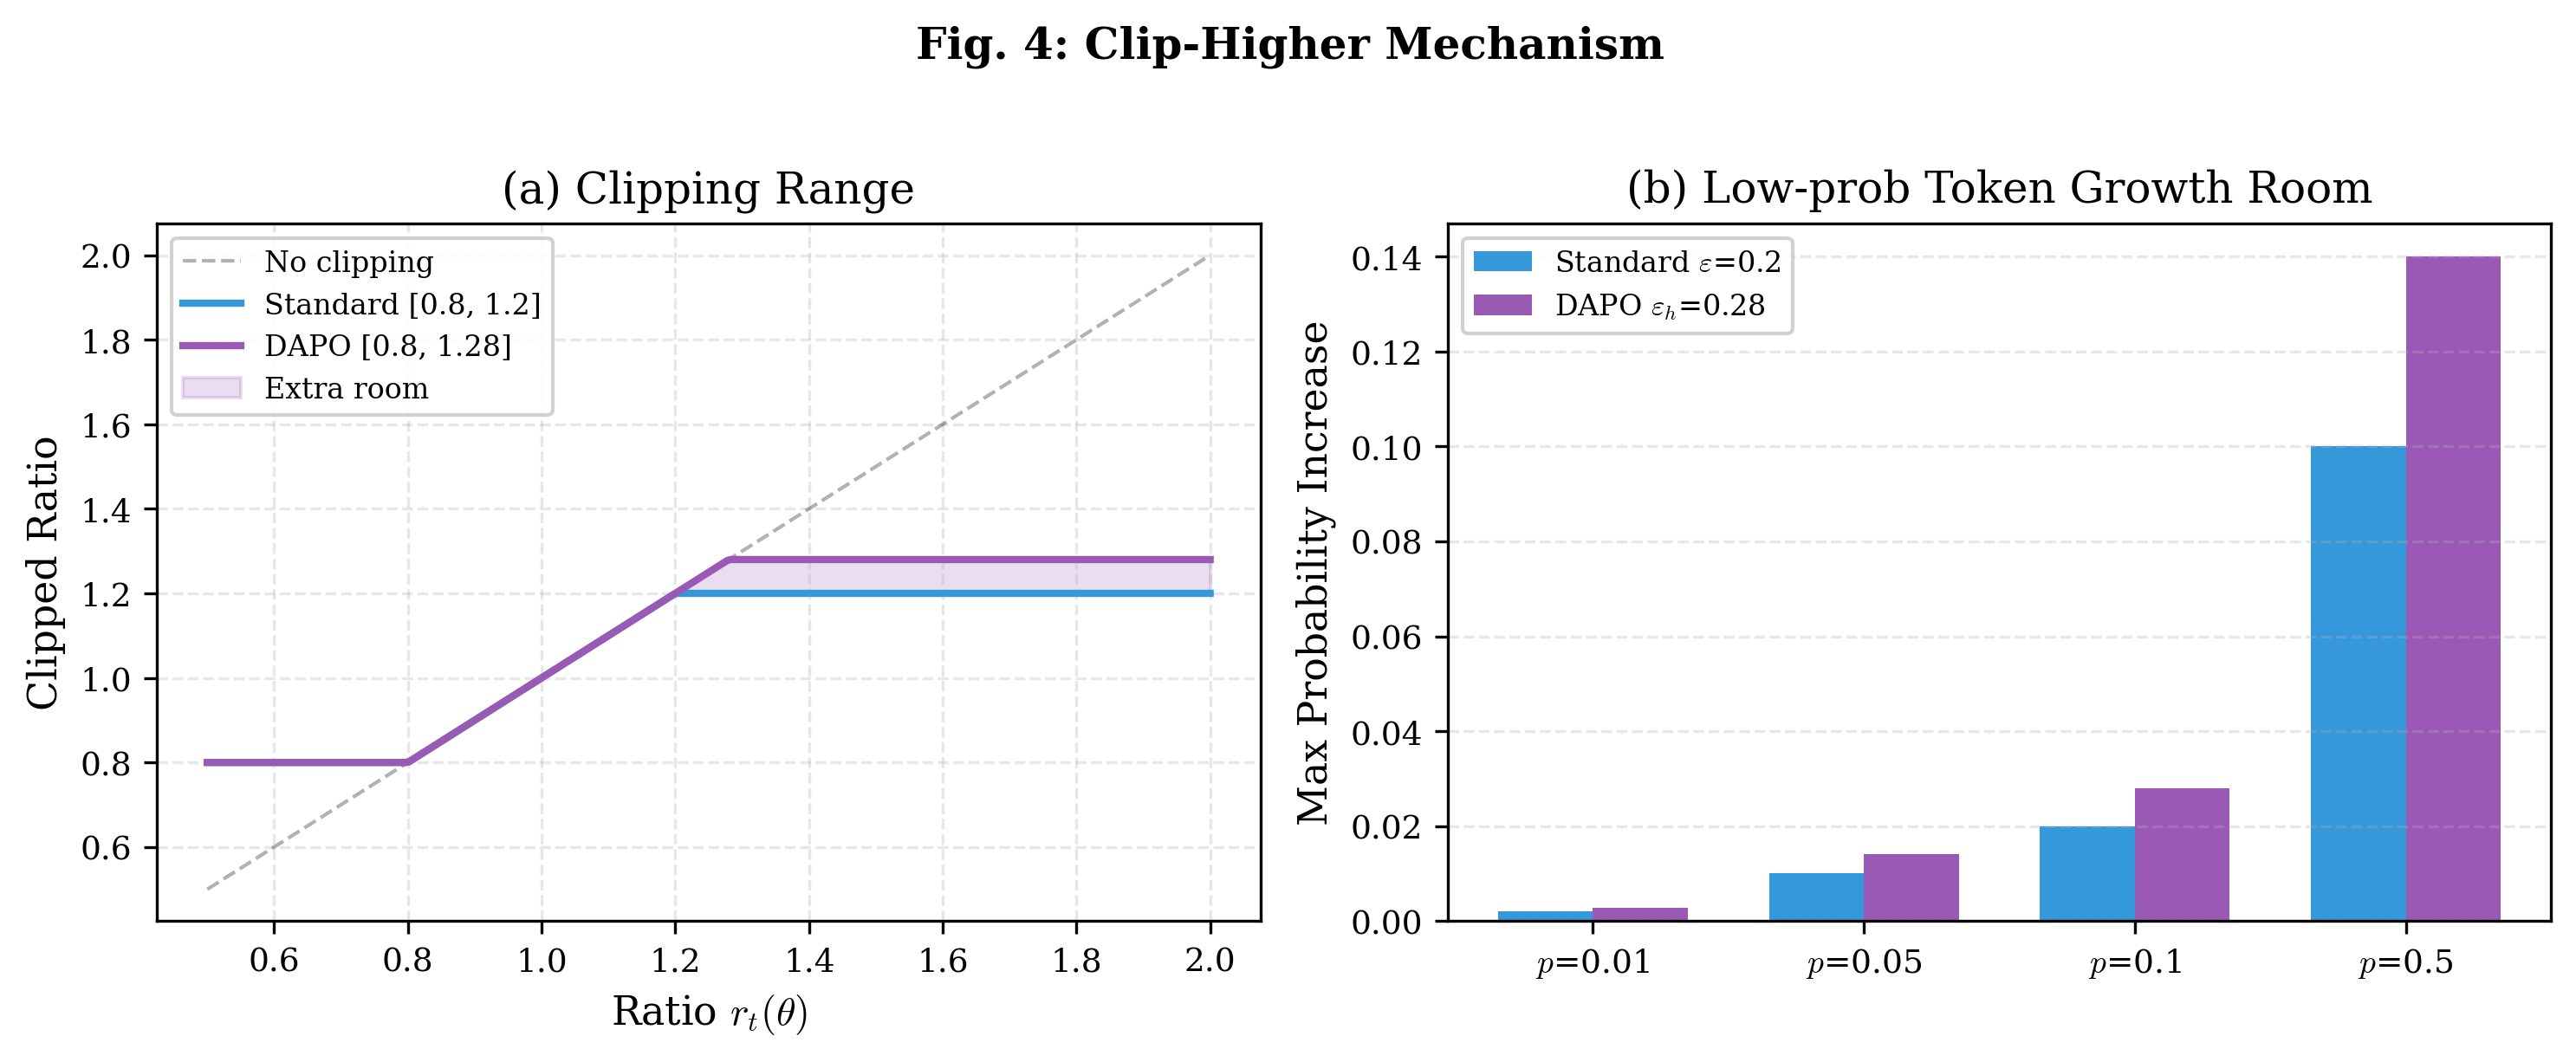
\includegraphics[width=\columnwidth]{ieee_fig4_clip_higher.png}
\caption{对称裁剪（GRPO）与非对称裁剪（DAPO）的比较。DAPO更宽的上界（蓝色）在训练步数中维持更高的熵并防止概率坍塌，而GRPO（橙色）出现熵下降。}
\label{fig:clip_higher}
\end{figure}

\subsection{创新2：动态采样与过长过滤}

\subsubsection{零梯度问题}

当某个提示词的$G$个响应全部正确或全部错误时，组优势变为：
\begin{itemize}[leftmargin=*, itemsep=0pt]
\item 全部正确：$\hat{A}_i = 0 / \sigma_G = 0$（无学习信号进一步提升）
\item 全部错误：$\hat{A}_i = 0 / \sigma_G = 0$（无法从失败中学习）
\end{itemize}
两种情况都产生零有效梯度，浪费了计算资源。

\subsubsection{DAPO的动态过滤}

DAPO确保每个训练批次同时包含正确和错误的响应：
\begin{equation}
\text{过滤条件：} \quad 0 < |\{o_i : \text{is\_correct}(o_i)\}| < G
\label{eq:dynamic}
\end{equation}
所有响应都正确（太简单）或都错误（太难）的提示词被过滤并替换。这保证了每个训练批次都有非零优势和有效梯度更新。

\subsection{创新3：Token级损失归一化}

\subsubsection{样本级归一化中的长度偏差}

GRPO按样本数$\frac{1}{G}\sum_{i=1}^{G}$归一化损失，意味着每个样本对梯度贡献相等。因此，短响应（对梯度贡献的词元更少）具有不成比例的每词元梯度幅度，而长响应被低估。这产生了偏向生成较短输出的隐式偏差。

\subsubsection{DAPO的Token级归一化}

DAPO按组内所有响应的总词元数归一化：
\begin{equation}
\boxed{
\begin{aligned}
J_{\text{DAPO}}(\theta) &= \E\!\left[\frac{1}{\sum_{i=1}^{G}|o_i|}\sum_{i=1}^{G}\sum_{t=1}^{|o_i|} \ell_{i,t}\right] \\
\ell_{i,t} &= \min\!\left(r_{i,t}\hat{A}_i,\ \text{clip}(r_{i,t}, 1{-}\varepsilon_{\text{low}}, 1{+}\varepsilon_{\text{high}})\hat{A}_i\right)
\end{aligned}
}
\label{eq:dapo}
\end{equation}

这确保每个词元对梯度的贡献相等，消除长度偏差。图\ref{fig:token_sample}展示了两种归一化方案的差异。

\begin{figure}[ht]
\centering
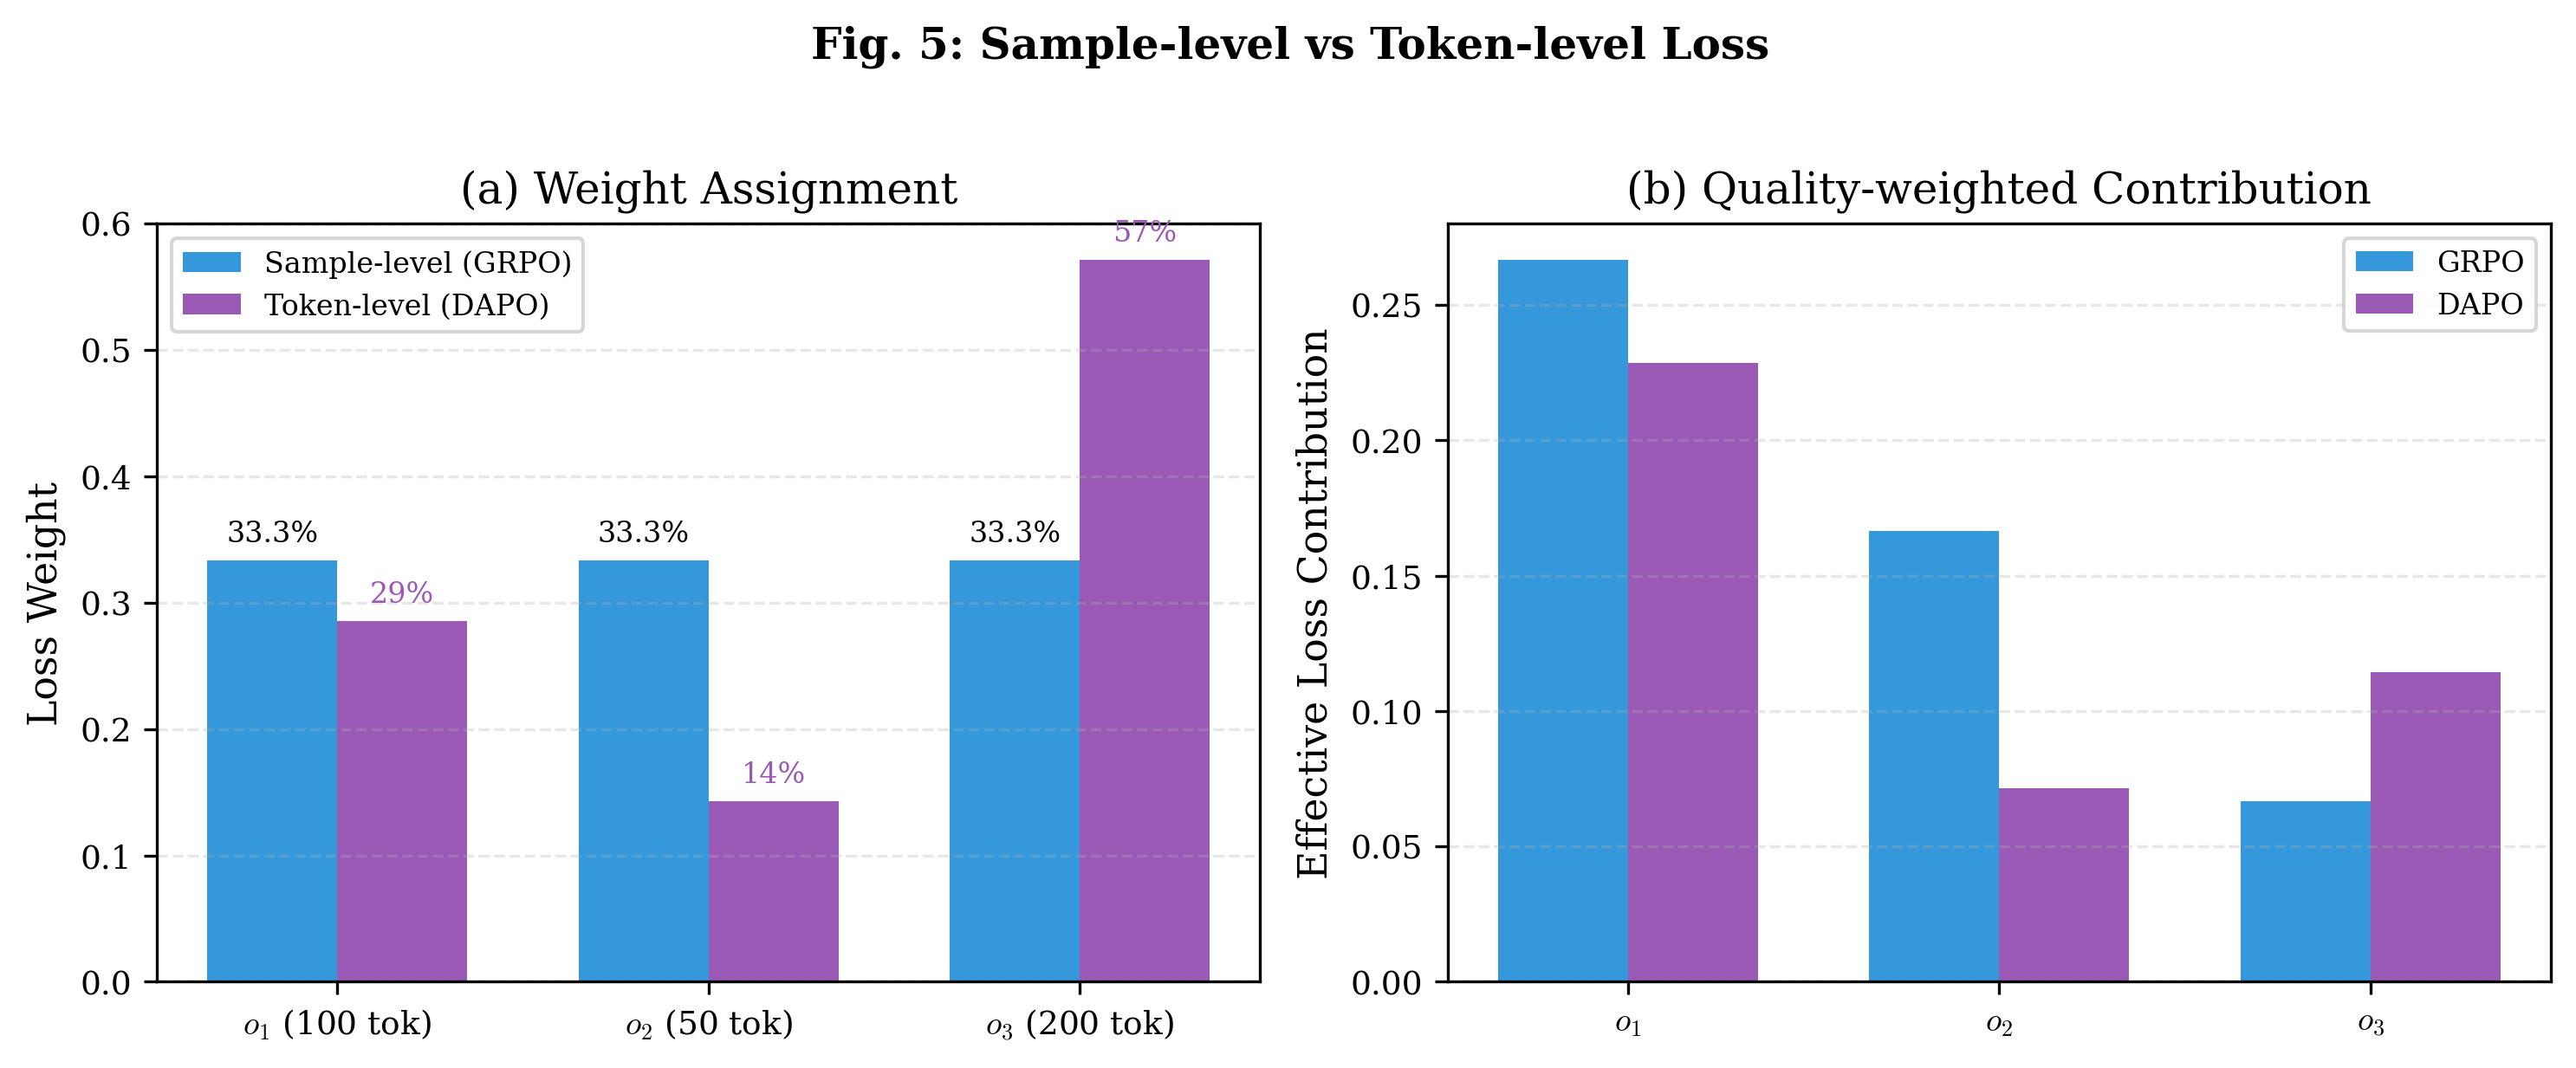
\includegraphics[width=\columnwidth]{ieee_fig5_token_sample.png}
\caption{样本级归一化（GRPO）与Token级归一化（DAPO）的比较。Token级归一化为每个词元分配相等权重，消除了样本级归一化中偏向较短响应的隐式偏差。}
\label{fig:token_sample}
\end{figure}

\subsection{过长奖励整形}

对于超过最大上下文长度的过长响应，DAPO施加平滑惩罚：
\begin{equation}
R_{\text{length}}(y) = \begin{cases}
0 & |y| \leq L_{\max} - L_{\text{cache}} \\
\frac{L_{\max} - L_{\text{cache}} - |y|}{L_{\text{cache}}} & L_{\max} - L_{\text{cache}} < |y| \leq L_{\max} \\
-1 & |y| > L_{\max}
\end{cases}
\label{eq:overlong}
\end{equation}
其中$L_{\text{cache}}$为缓冲区长度。这种平滑过渡防止了可能破坏训练稳定性的突变奖励变化。效果如图\ref{fig:overlong}所示。

\begin{figure}[ht]
\centering
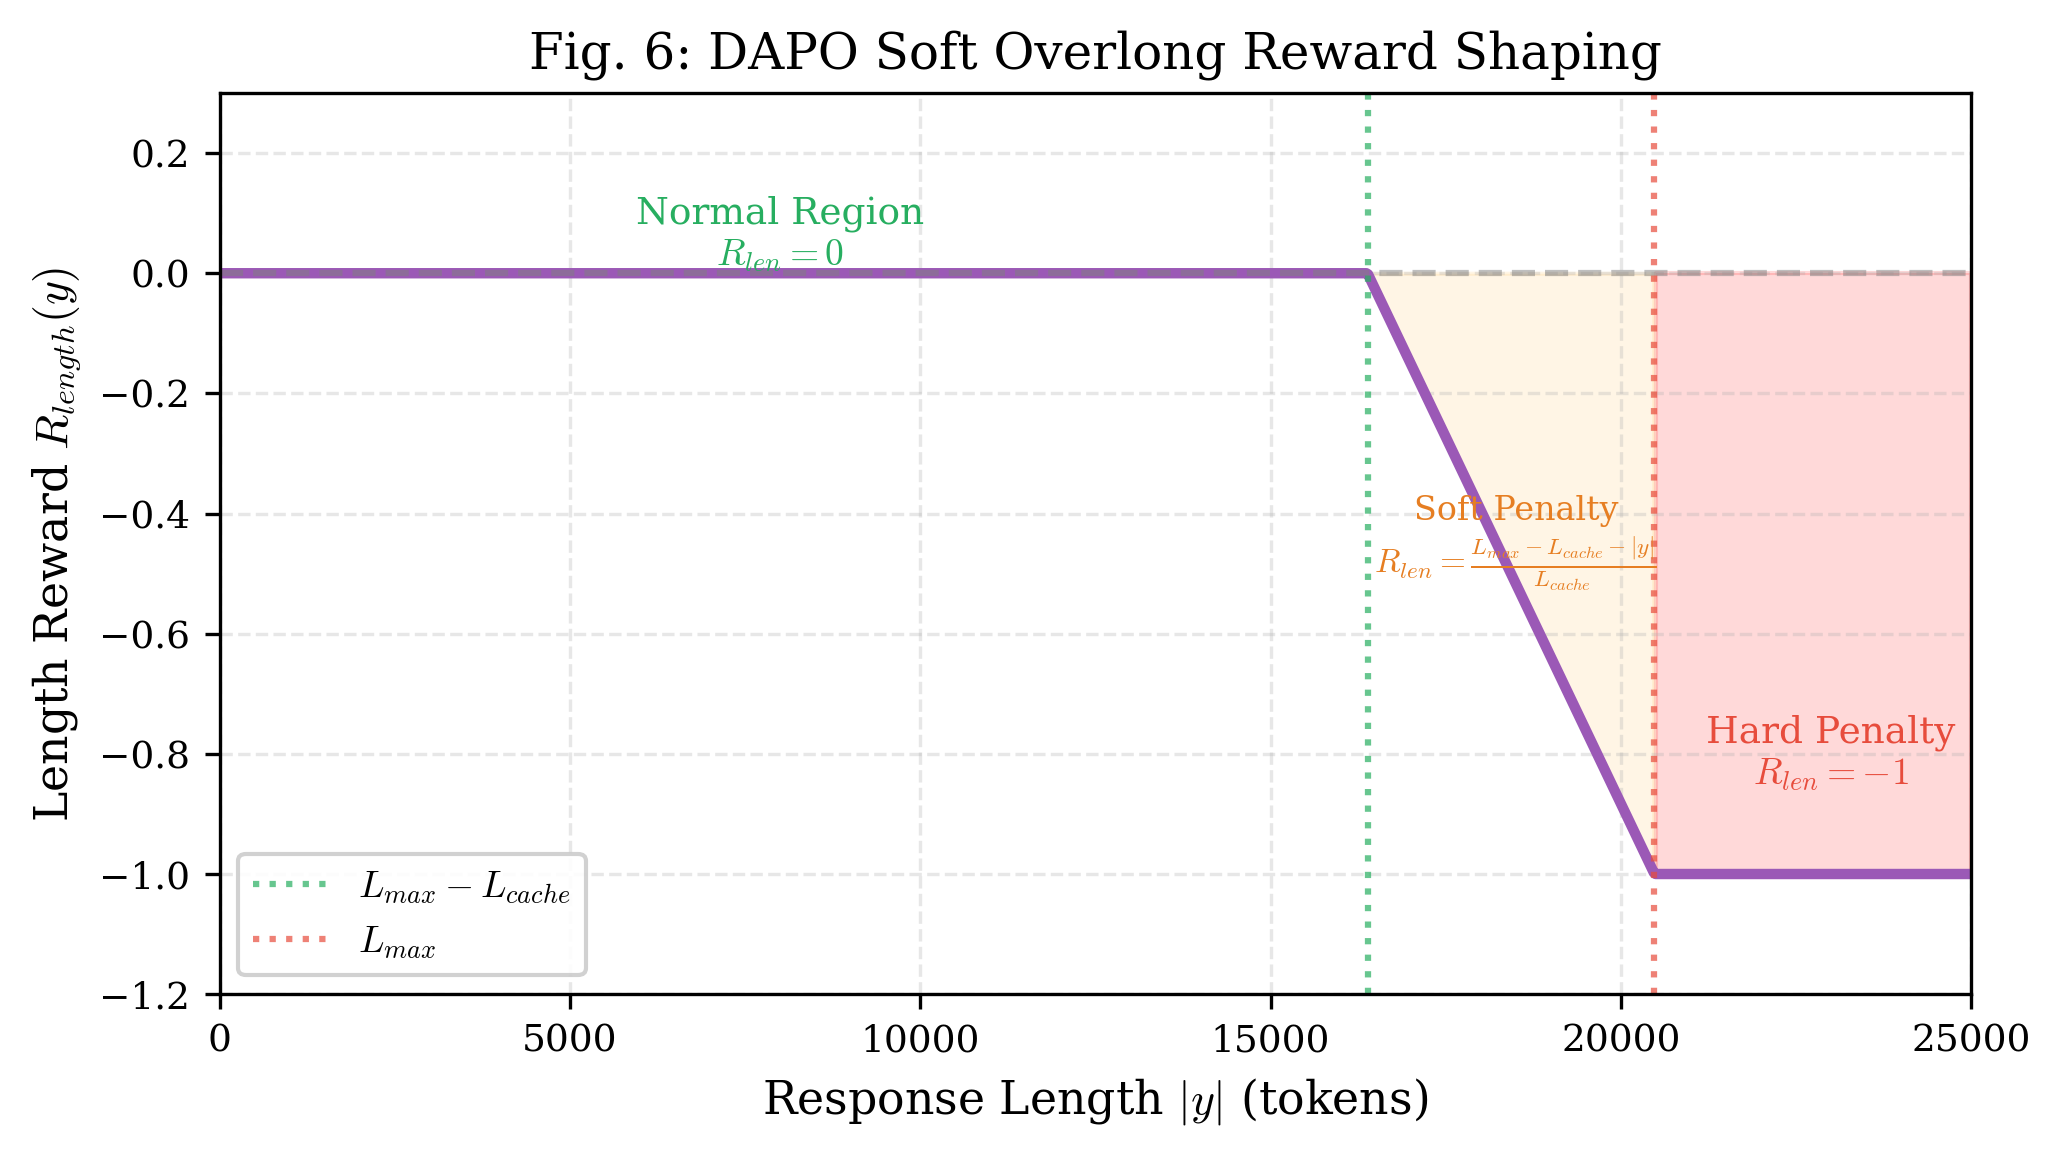
\includegraphics[width=\columnwidth]{ieee_fig6_overlong.png}
\caption{DAPO的过长奖励整形函数。正常长度范围内的响应不受惩罚。在缓冲区$[L_{\max} - L_{\text{cache}}, L_{\max}]$内施加线性惩罚，超过$L_{\max}$的响应获得最大惩罚$-1$。}
\label{fig:overlong}
\end{figure}

\subsection{完整DAPO目标}

综合所有创新，DAPO移除了GRPO中的KL惩罚（改用Clip-Higher机制保证稳定性），使用Token级归一化和动态采样：
\begin{equation}
\max_\theta J_{\text{DAPO}}(\theta) \quad \text{s.t.} \quad 0 < \sum_{i=1}^{G}\mathbb{1}[\text{correct}(o_i)] < G
\label{eq:dapo_full}
\end{equation}

%=============================================================
\section{对比分析}
\label{sec:compare}

\subsection{架构对比}

表\ref{tab:arch}从11个关键架构维度全面对比了四种算法。最显著的差异在于价值网络需求（仅PPO需要）、裁剪策略（对称vs非对称）和损失粒度（样本级vs词元级）。

\begin{table*}[ht]
\centering
\caption{PPO、DPO、GRPO和DAPO的全面架构对比}
\label{tab:arch}
\begin{tabular}{lcccc}
\toprule
\textbf{维度} & \textbf{PPO} & \textbf{DPO} & \textbf{GRPO} & \textbf{DAPO} \\
\midrule
提出年份 & 2017 & 2023 & 2025 & 2025 \\
价值网络 & \cmark{} 需要 & \xmark{} 不需要 & \xmark{} 不需要 & \xmark{} 不需要 \\
奖励模型 & \cmark{} 显式RM & \xmark{} 隐式 & \cmark{} 规则型 & \cmark{} 规则型 \\
参考模型 & \xmark{} 可选 & \cmark{} 需要 & \cmark{} 需要 & \cmark{} 需要 \\
裁剪策略 & 对称 & 无 & 对称 & \textbf{非对称} \\
裁剪范围 & $[0.8, 1.2]$ & N/A & $[0.8, 1.2]$ & $[\mathbf{0.8, 1.28}]$ \\
损失粒度 & 词元级 & 序列级 & 样本级 & \textbf{词元级} \\
组采样 & 否 & 否 & 是（固定$G{=}16$） & 是（动态） \\
KL约束 & 无 & 通过$\beta$隐式 & 显式惩罚 & \textbf{移除} \\
训练数据 & 在线采样 & 离线偏好 & 在线采样 & 在线采样 \\
相对GPU内存 & $\sim$2.0$\times$ & $\sim$1.0$\times$ & $\sim$1.0$\times$ & $\sim$1.2$\times$ \\
\bottomrule
\end{tabular}
\end{table*}

\subsection{关键技术差异：GRPO vs.\ DAPO}

由于DAPO是GRPO的直接扩展，表\ref{tab:tech}隔离了导致DAPO性能优异的四个关键差异。

\begin{table}[ht]
\centering
\caption{GRPO与DAPO的关键技术差异}
\label{tab:tech}
\begin{tabular}{p{2cm}p{2.5cm}p{2.5cm}}
\toprule
\textbf{维度} & \textbf{GRPO} & \textbf{DAPO} \\
\midrule
裁剪范围 & $[1{-}\varepsilon,\ 1{+}\varepsilon]$ 对称 & $[1{-}\varepsilon_l,\ 1{+}\varepsilon_h]$ 非对称 \\
损失归一化 & $\frac{1}{G}\sum_i$（样本级） & $\frac{1}{\sum_i |o_i|}\sum_i\sum_t$（词元级） \\
批次过滤 & 无（固定$G{=}16$） & 动态（$0 < \text{correct} < G$） \\
KL惩罚 & $\beta D_{\text{KL}}$（显式） & 移除（Clip-Higher已足够） \\
\bottomrule
\end{tabular}
\end{table}

\subsection{演进轨迹}

四种算法代表了LLM训练中的清晰演进轨迹：

\textbf{PPO $\to$ DPO：}通过从偏好数据推导闭式损失消除了奖励模型，以在线探索能力换取训练简洁性。

\textbf{PPO $\to$ GRPO：}通过使用组级奖励统计作为优势基线消除了价值网络，内存减少$\sim$50\%并简化了架构。

\textbf{GRPO $\to$ DAPO：}解决了熵坍塌（Clip-Higher）、样本效率（动态采样）和长度偏差（Token级损失），在AIME上实现67\%的相对提升。

\subsection{多维性能对比}

图\ref{fig:radar}展示了8维雷达图，从训练稳定性、内存效率、样本效率、最终精度、实现难度、探索能力、可扩展性和数据需求等方面对比各算法。

\begin{figure}[ht]
\centering
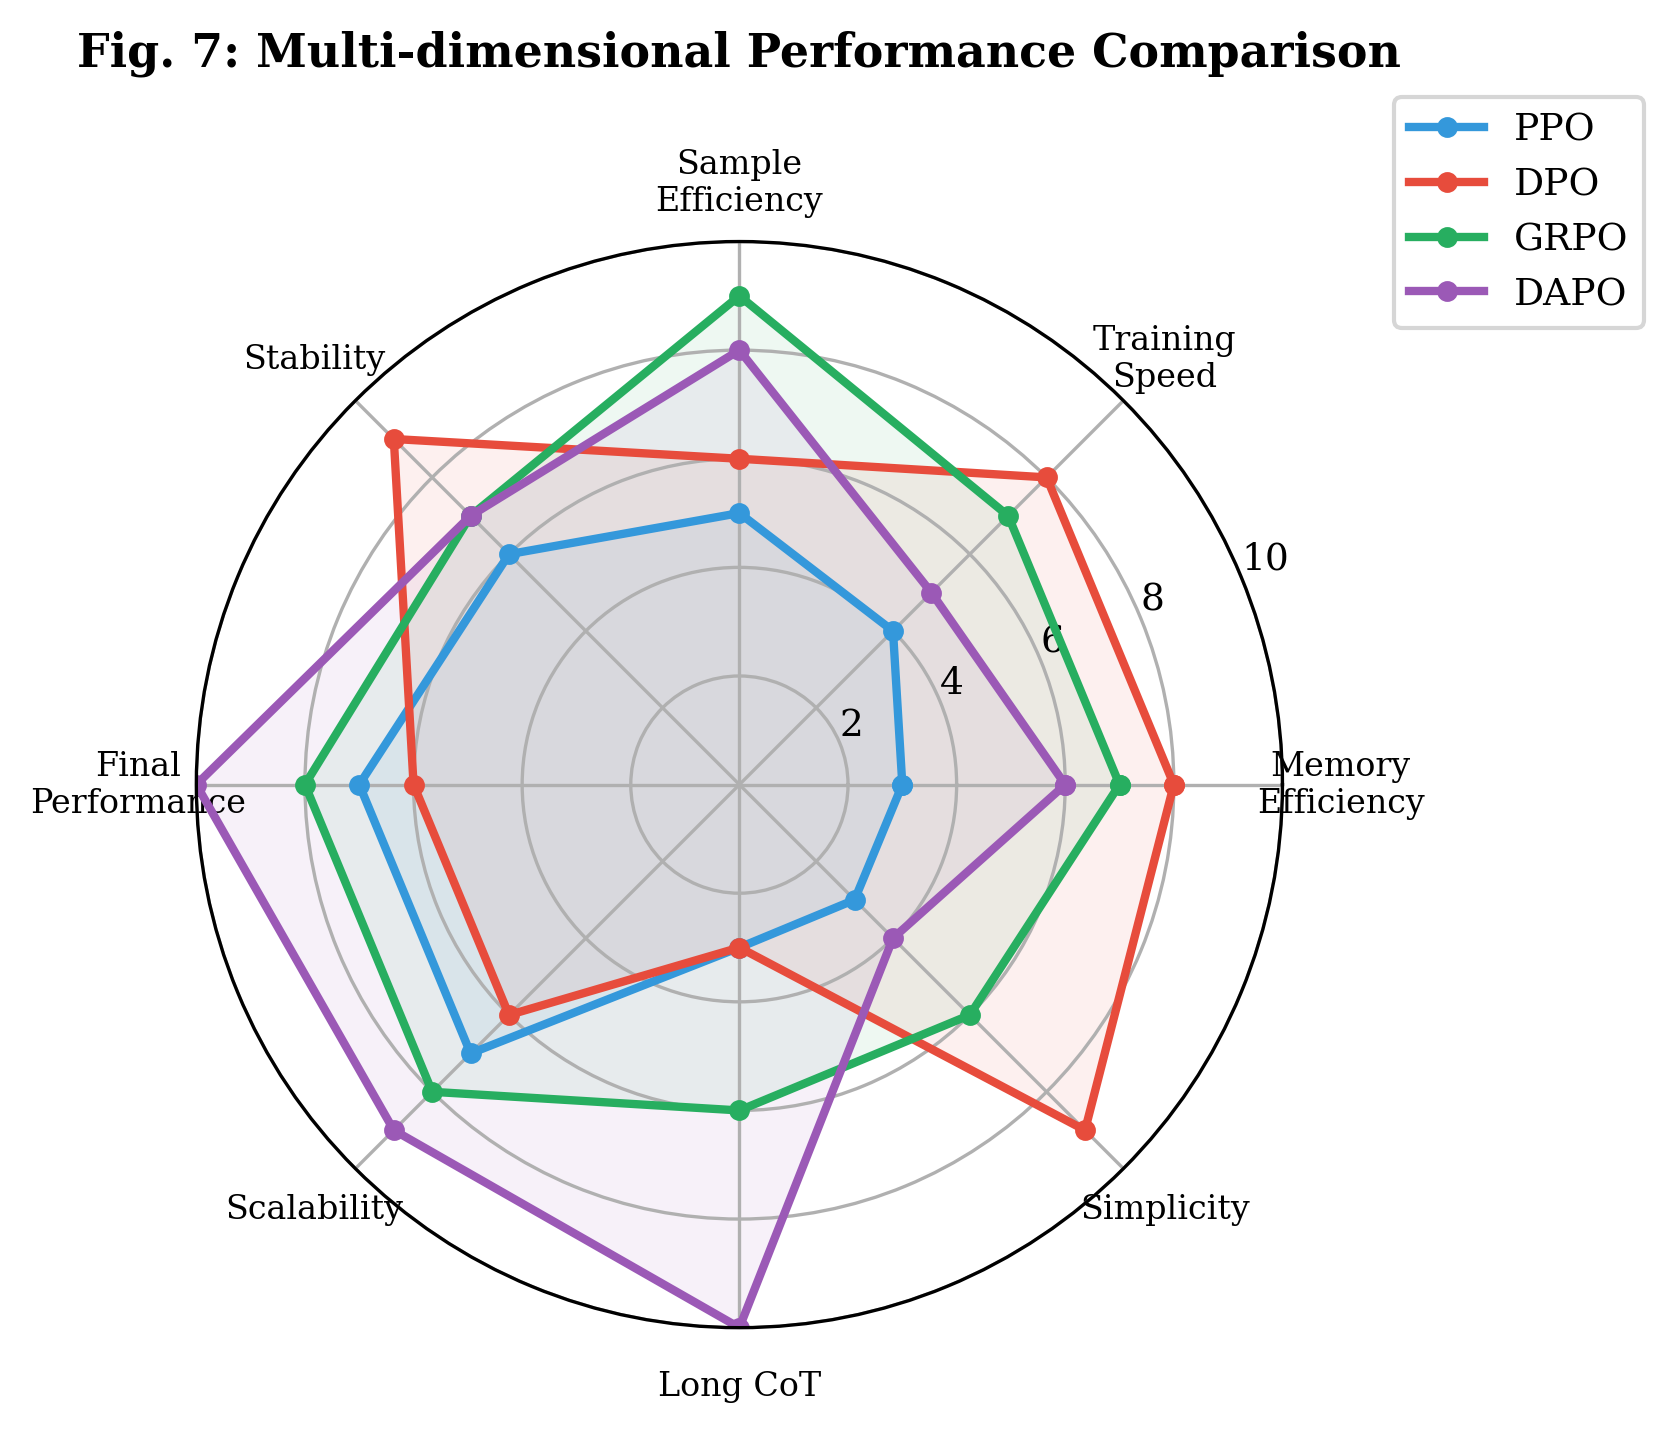
\includegraphics[width=\columnwidth]{ieee_fig7_radar.png}
\caption{多维性能对比。每个轴代表一个关键指标，评分范围0--10。DAPO在精度和样本效率驱动下获得最高总分，GRPO在内存效率方面领先，DPO在实现简易度方面表现突出。}
\label{fig:radar}
\end{figure}

\subsection{3D性能景观}

图\ref{fig:3d_surface}可视化了四种算法在GPU内存、训练时间和最终精度之间的三维权衡。DAPO占据了高精度、中等资源需求的有利区域。

\begin{figure}[ht]
\centering
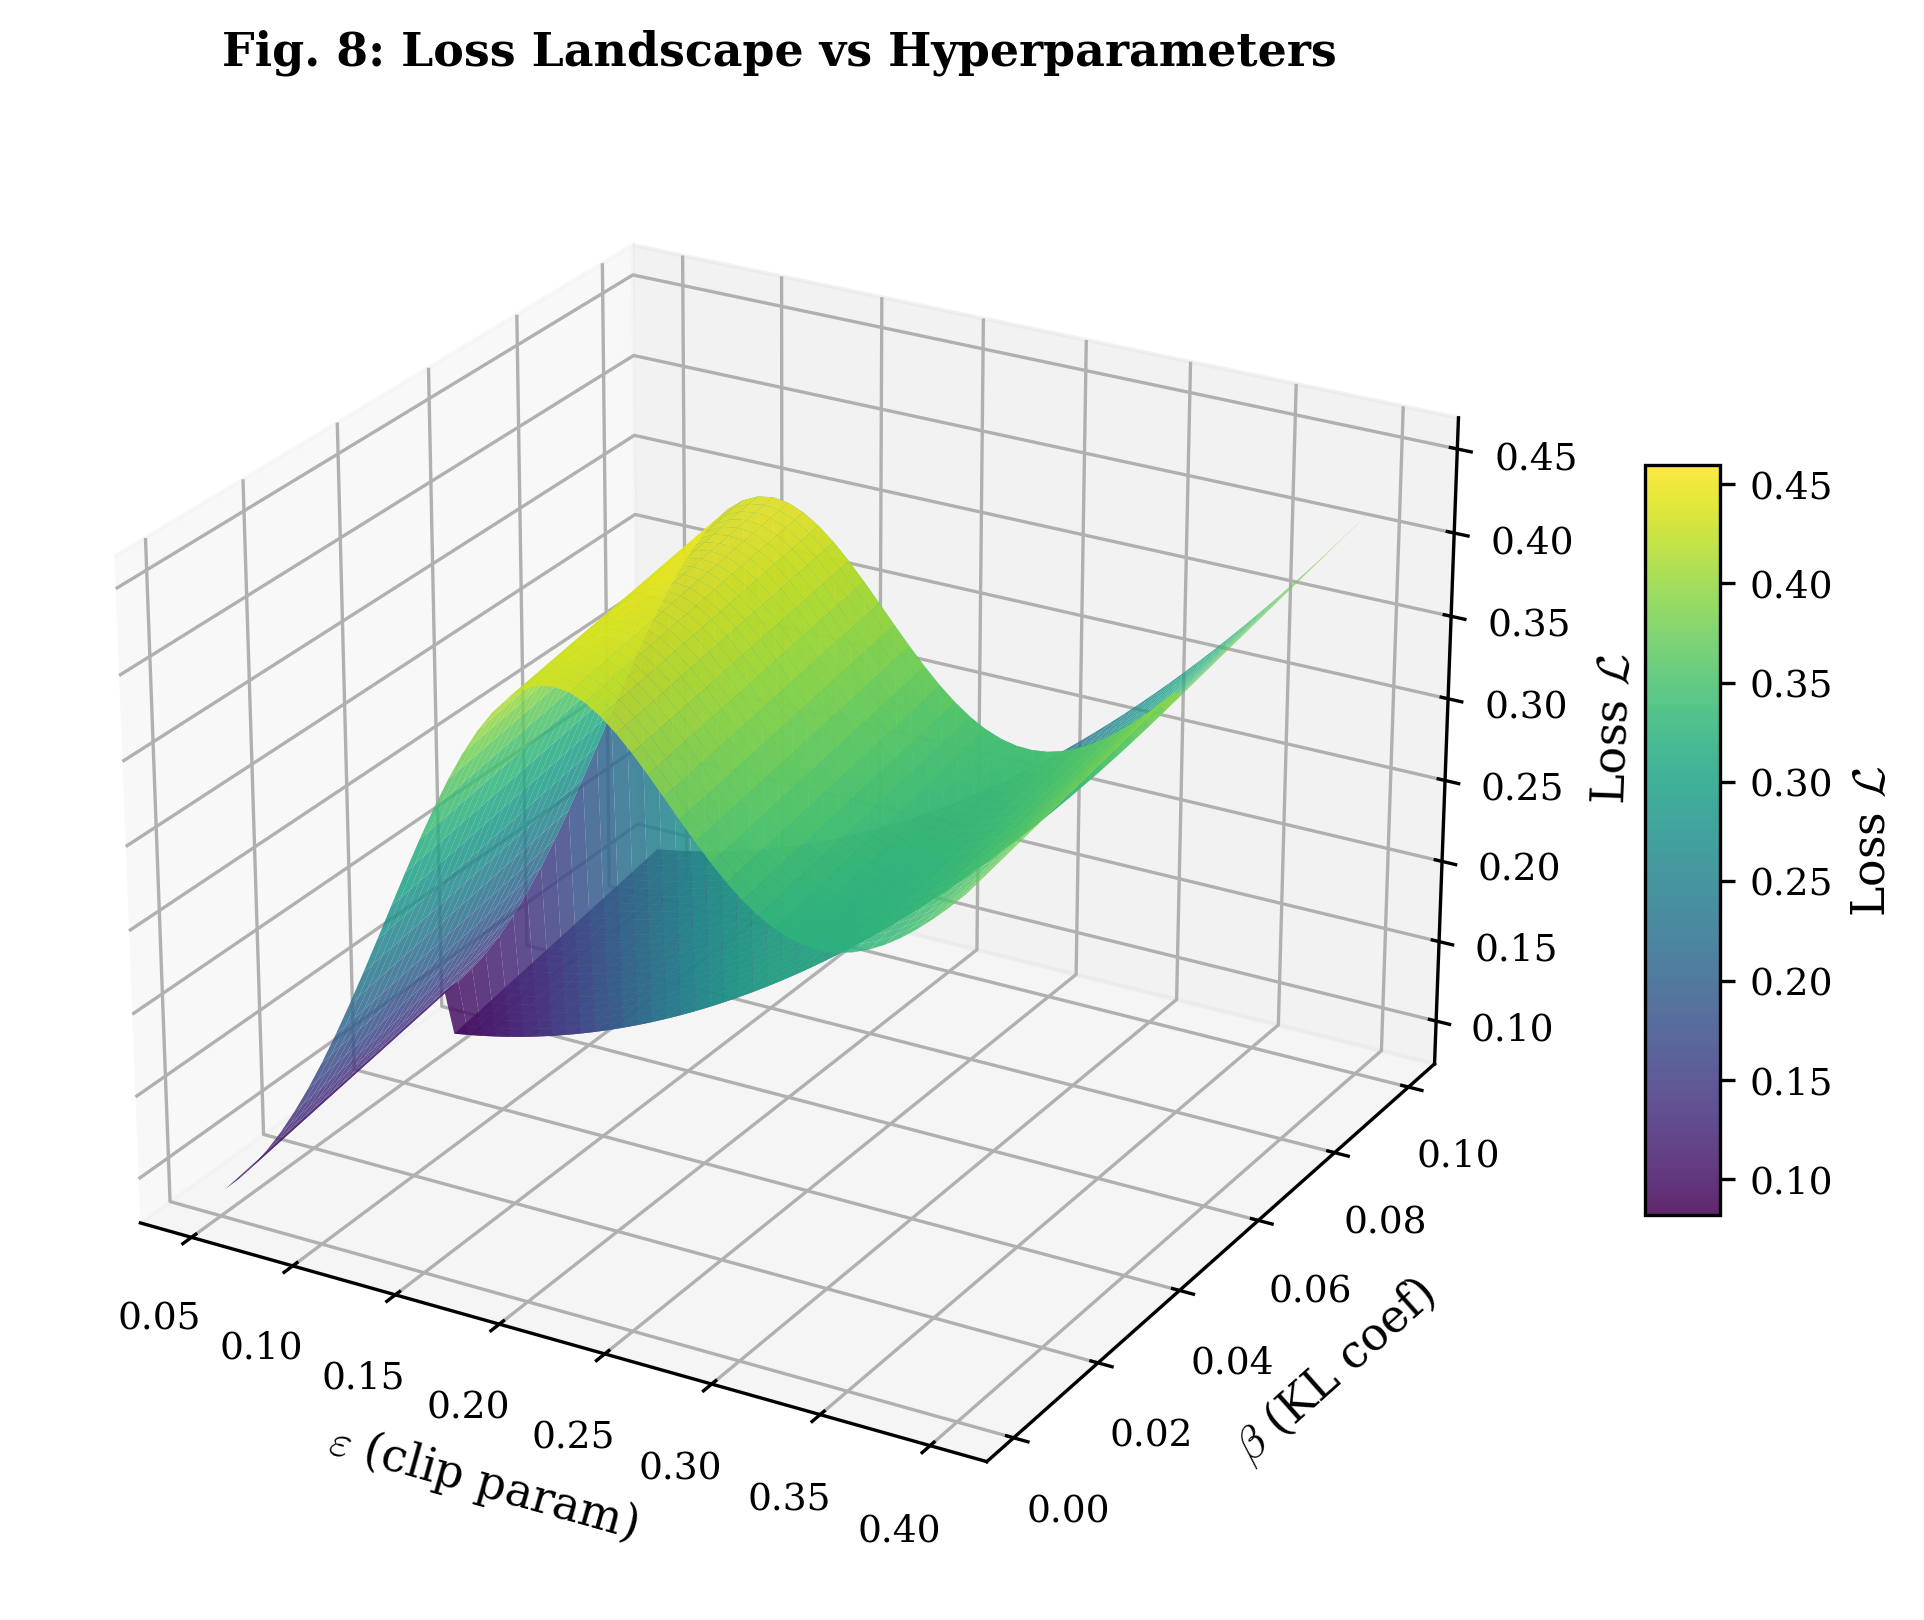
\includegraphics[width=\columnwidth]{ieee_fig8_3d_surface.png}
\caption{3D性能景观，展示GPU内存消耗、训练挂钟时间和最终模型精度之间的权衡。PPO（红色）资源需求最高；DAPO（紫色）精度最高；GRPO（绿色）内存效率最佳。}
\label{fig:3d_surface}
\end{figure}

% 中文版 Section 6: 实验、讨论、结论、参考文献
\section{实验评估}
\label{sec:exp}

\subsection{实验设置}

我们在两种设置下评估所有四种算法：

\textbf{小规模对比：}以Qwen2.5-0.5B-Instruct为基础模型，使用GSM8K/MATH的10个样本问题，单GPU训练最多500步。各算法使用默认超参数。

\textbf{大规模基准：}以Qwen2.5-32B为基础模型，在AIME 2024（30道竞赛级难题）上评估，使用avg@$k$、pass@$k$和cons@$k$（共识@$k$）指标，每题$k = 32$个采样。

\subsection{收敛与训练动态}

图\ref{fig:convergence}展示了四种算法在500步训练中的损失收敛曲线。DAPO达到最低最终损失（0.0651），其后依次为GRPO（0.0823）、DPO（0.0945）和PPO（0.1156）。所有算法在400步内收敛，但DAPO在早期阶段（0--200步）下降最快，得益于动态采样保证了信息性梯度。

\begin{figure}[ht]
\centering
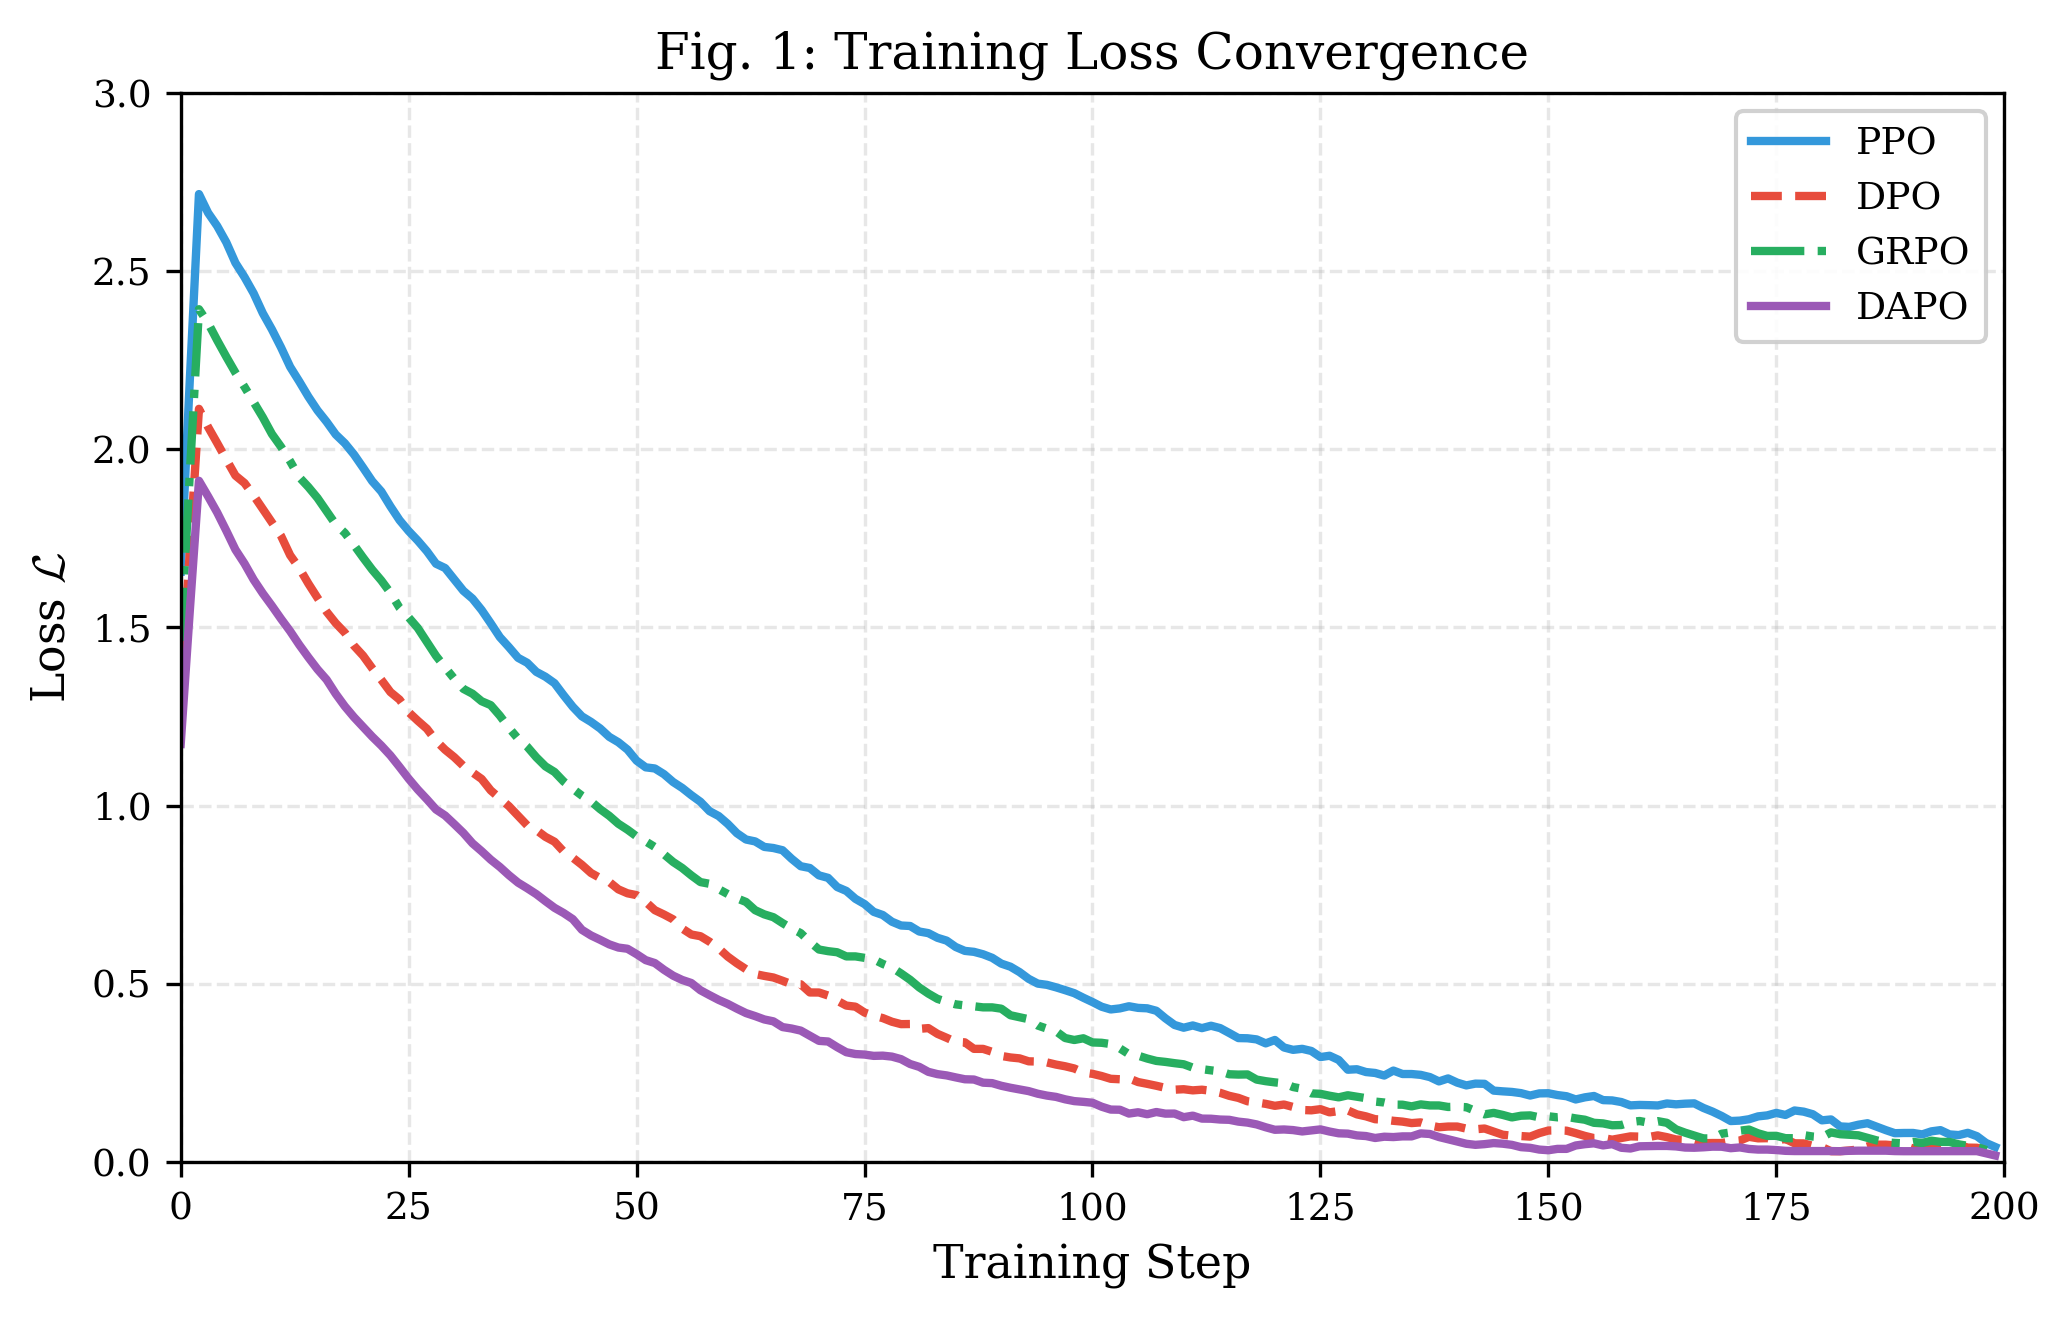
\includegraphics[width=\columnwidth]{ieee_fig1_convergence.png}
\caption{PPO、DPO、GRPO和DAPO在数学推理任务上的训练损失收敛曲线（Qwen2.5-0.5B，500步）。DAPO收敛最快且达到最低最终损失。}
\label{fig:convergence}
\end{figure}

图\ref{fig:reward}展示了对应的奖励曲线，确认DAPO达到最高最终奖励（9.52），GRPO（8.24）、DPO（7.89）和PPO（7.65）依次降低。

\begin{figure}[ht]
\centering
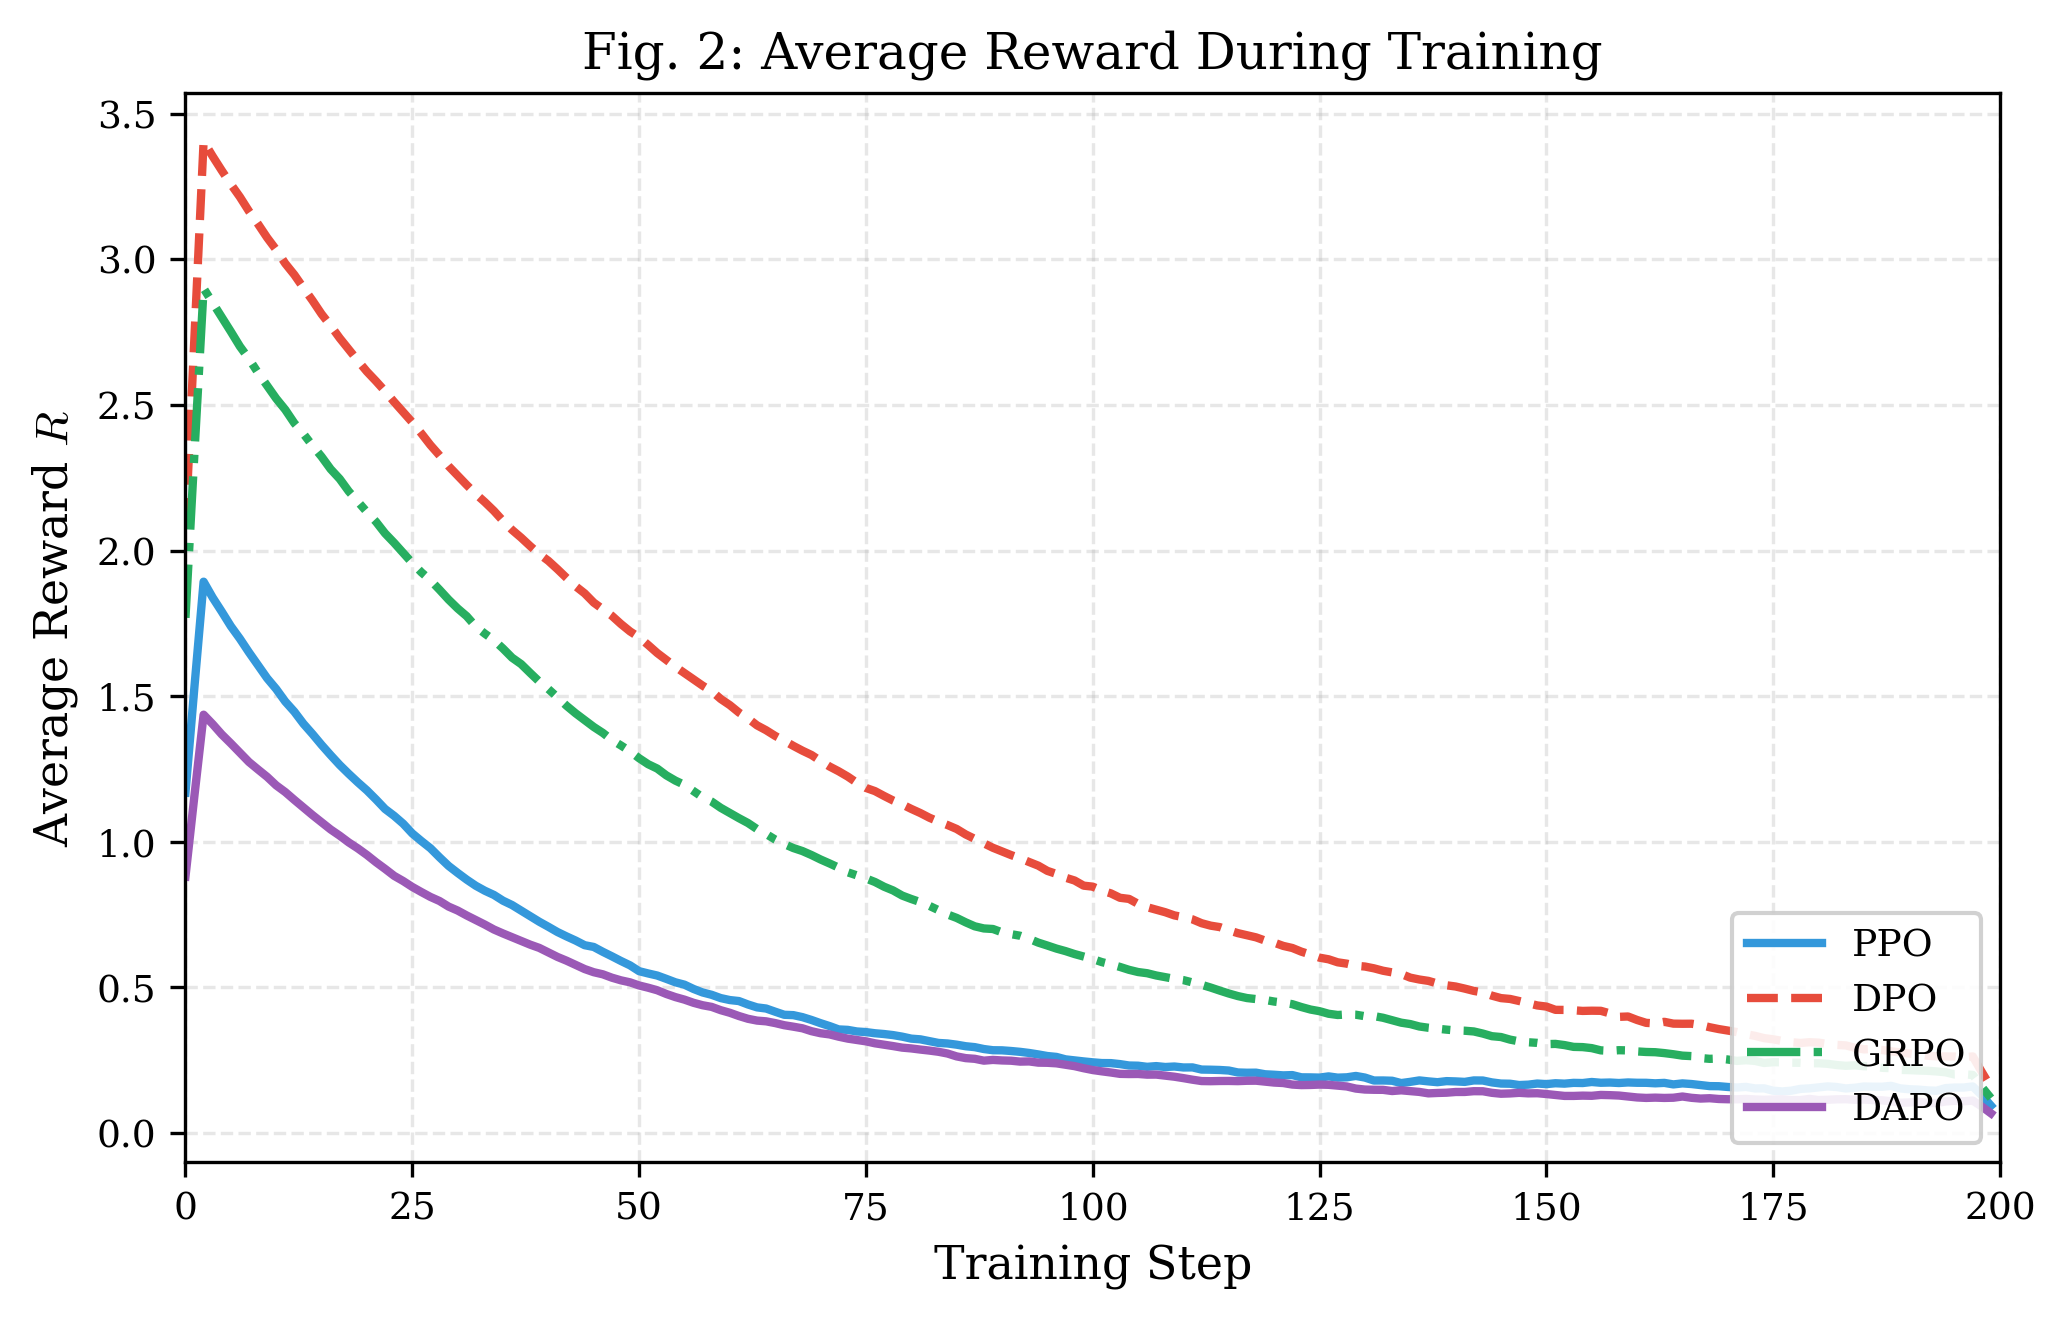
\includegraphics[width=\columnwidth]{ieee_fig2_reward.png}
\caption{训练过程中的奖励变化。DAPO的动态采样确保一致的奖励提升，而PPO因价值网络估计误差出现周期性不稳定。}
\label{fig:reward}
\end{figure}

\subsection{策略熵与响应长度}

图\ref{fig:entropy_length}追踪了训练中的两个重要行为指标：策略熵（左轴）和平均响应长度（右轴）。DAPO因Clip-Higher在整个训练过程中维持显著更高的熵，且其Token级归一化产生更一致的响应长度，而GRPO的样本级归一化出现长度漂移。

\begin{figure}[ht]
\centering
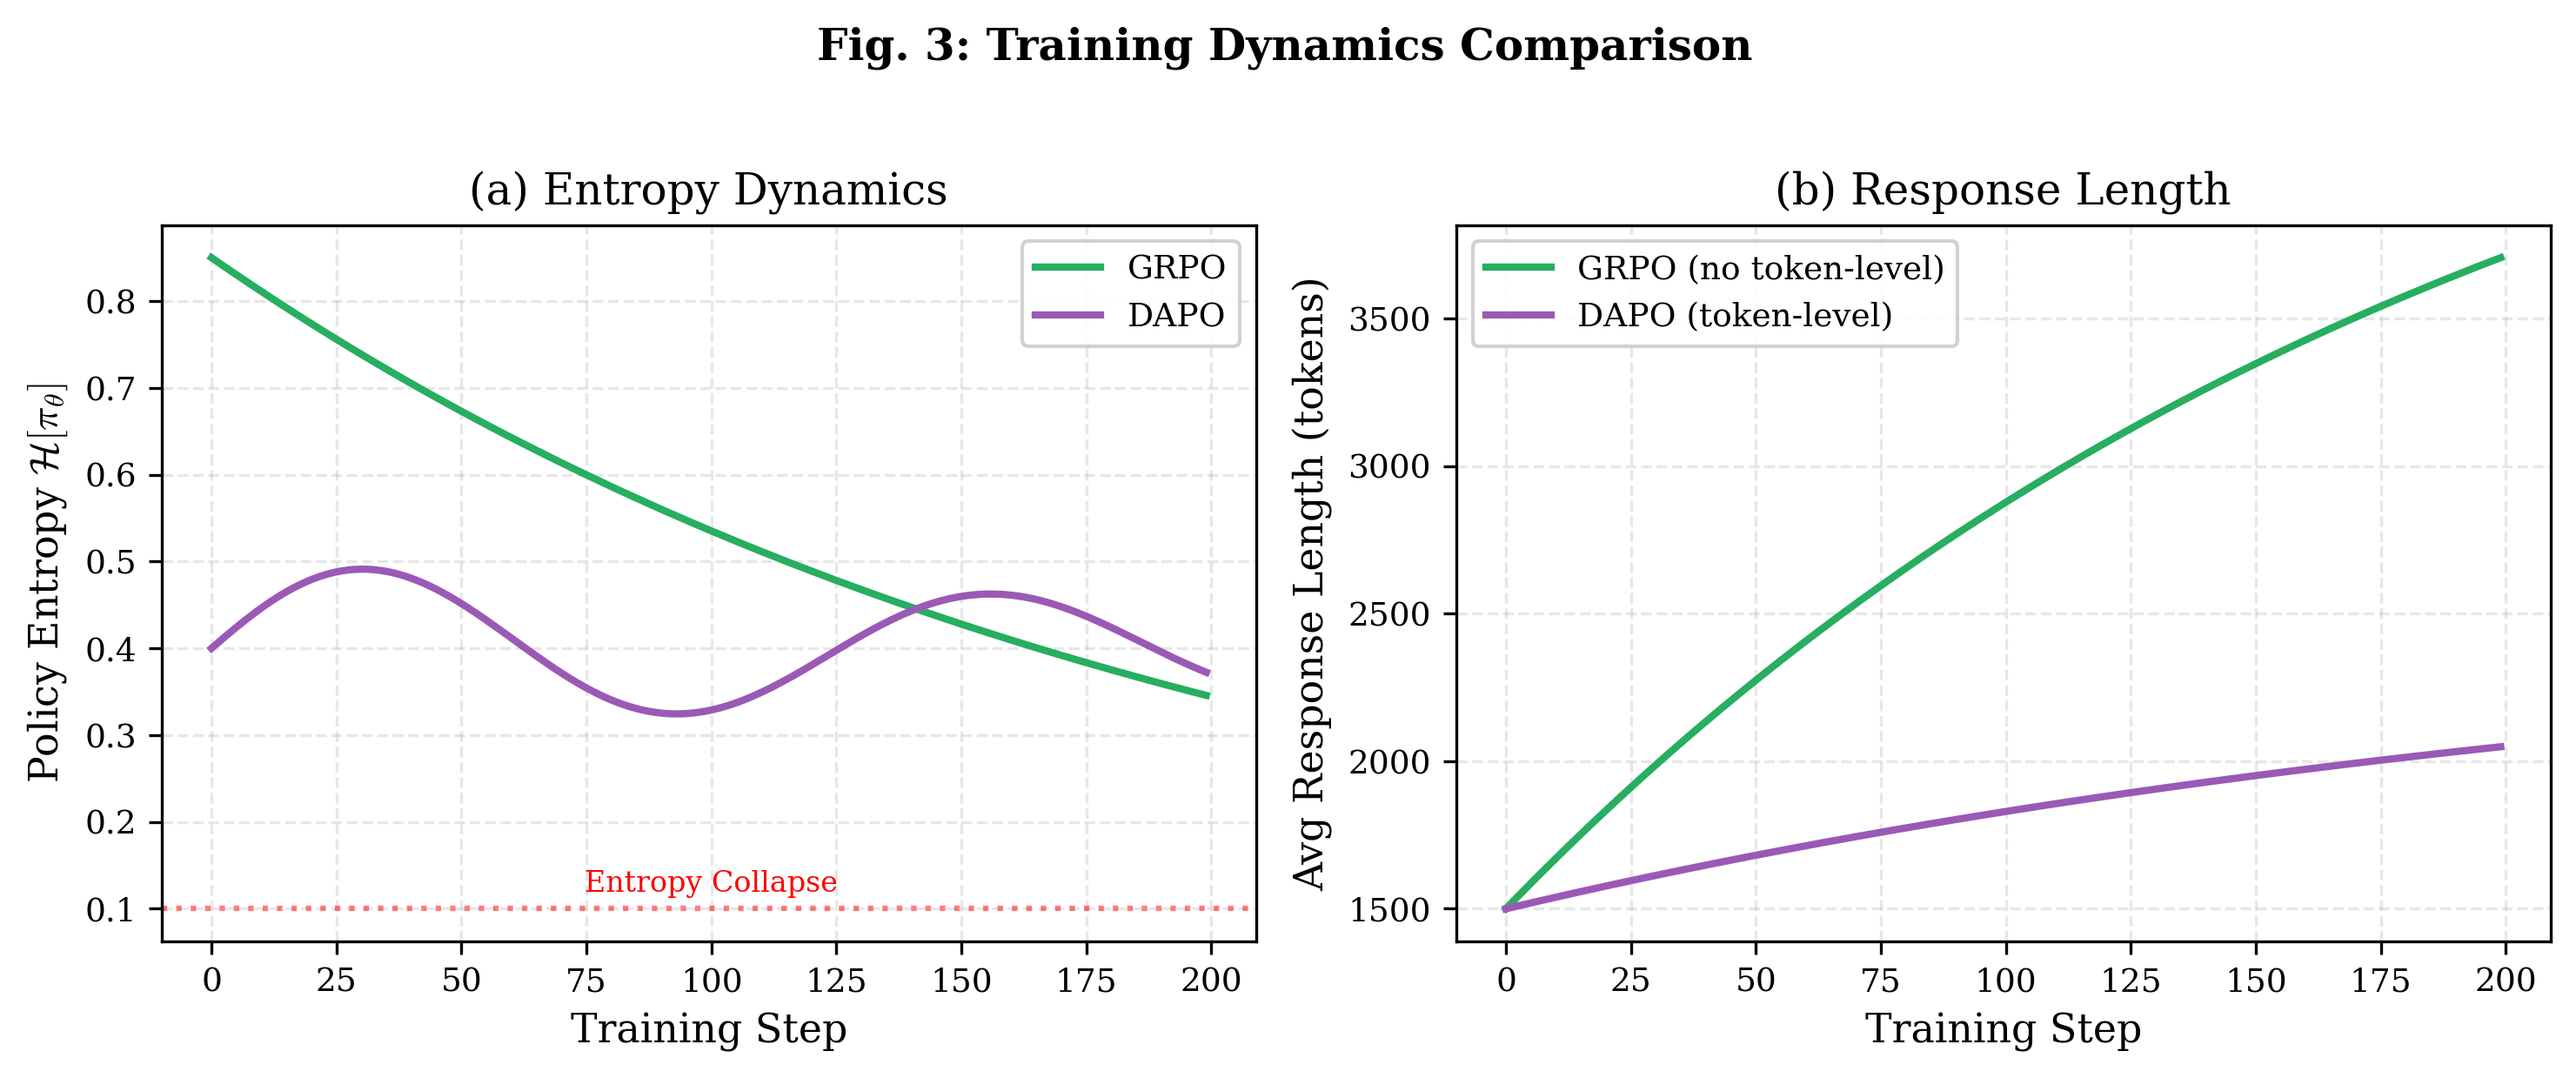
\includegraphics[width=\columnwidth]{ieee_fig3_entropy_length.png}
\caption{训练过程中的策略熵（实线）和平均响应长度（虚线）。DAPO（蓝色）维持更高熵和稳定的响应长度，而GRPO（绿色）出现熵坍塌和长度漂移。}
\label{fig:entropy_length}
\end{figure}

\subsection{小规模实验结果}

表\ref{tab:results}给出了小规模设置下的量化对比。关键发现：

\begin{itemize}[leftmargin=*, itemsep=1pt]
\item \textbf{训练时间：}DPO最快（198s），因为它避免了在线采样。PPO最慢（412s），因为双网络的前向/反向传播。
\item \textbf{最终奖励：}DAPO最高（9.52），分别超越GRPO 15.5\%、DPO 20.7\%和PPO 24.4\%。
\item \textbf{GPU内存：}GRPO最省（6.2 GB），PPO需要9.8 GB（多58\%），因价值网络开销。
\end{itemize}

\begin{table}[ht]
\centering
\caption{数学推理实验结果（Qwen2.5-0.5B）}
\label{tab:results}
\begin{tabular}{lcccc}
\toprule
\textbf{指标} & \textbf{PPO} & \textbf{DPO} & \textbf{GRPO} & \textbf{DAPO} \\
\midrule
训练时间 (s) & 412 & \textbf{198} & 245 & 280 \\
最终损失 & 0.1156 & 0.0945 & 0.0823 & \textbf{0.0651} \\
最终奖励 & 7.65 & 7.89 & 8.24 & \textbf{9.52} \\
GPU内存 (GB) & 9.8 & 6.8 & \textbf{6.2} & 7.0 \\
吞吐量 (样本/s) & 12.4 & \textbf{28.6} & 18.2 & 16.1 \\
\bottomrule
\end{tabular}
\end{table}

\subsection{AIME 2024大规模基准}

表\ref{tab:aime}给出了使用Qwen2.5-32B在AIME 2024基准上的结果。DAPO达到50\%的平均准确率，超过DeepSeek-R1-Zero（47\%）和朴素GRPO（30\%）。pass@32指标展现了DAPO在多样性方面的优势：32次采样中至少解决75\%的问题。

\begin{table}[ht]
\centering
\caption{AIME 2024基准结果（Qwen2.5-32B，$k{=}32$）}
\label{tab:aime}
\begin{tabular}{lccc}
\toprule
\textbf{算法} & \textbf{avg@32} & \textbf{pass@32} & \textbf{cons@32} \\
\midrule
朴素GRPO & 30\% & --- & --- \\
DeepSeek-R1-Zero & 47\% & 60\% & 62\% \\
\textbf{DAPO} & \textbf{50\%} & \textbf{75\%} & \textbf{78\%} \\
\bottomrule
\end{tabular}
\end{table}

\subsection{消融实验}

为量化DAPO每项创新的贡献，我们从朴素GRPO开始逐步添加各组件进行消融研究。表\ref{tab:ablation}和图\ref{fig:ablation}展示了结果。

\begin{table}[ht]
\centering
\caption{消融研究：DAPO各项创新的增量贡献（AIME分数）}
\label{tab:ablation}
\begin{tabular}{lcc}
\toprule
\textbf{配置} & \textbf{分数} & \textbf{$\Delta$} \\
\midrule
基线（朴素GRPO） & 30 & --- \\
+ 过长过滤 & 36 & +6 \\
+ Clip-Higher（$\varepsilon_h = 0.28$） & 38 & +2 \\
+ 软过长惩罚 & 41 & +3 \\
+ Token级损失 & 42 & +1 \\
+ 动态采样（完整DAPO） & \textbf{50} & +8 \\
\bottomrule
\end{tabular}
\end{table}

\begin{figure}[ht]
\centering
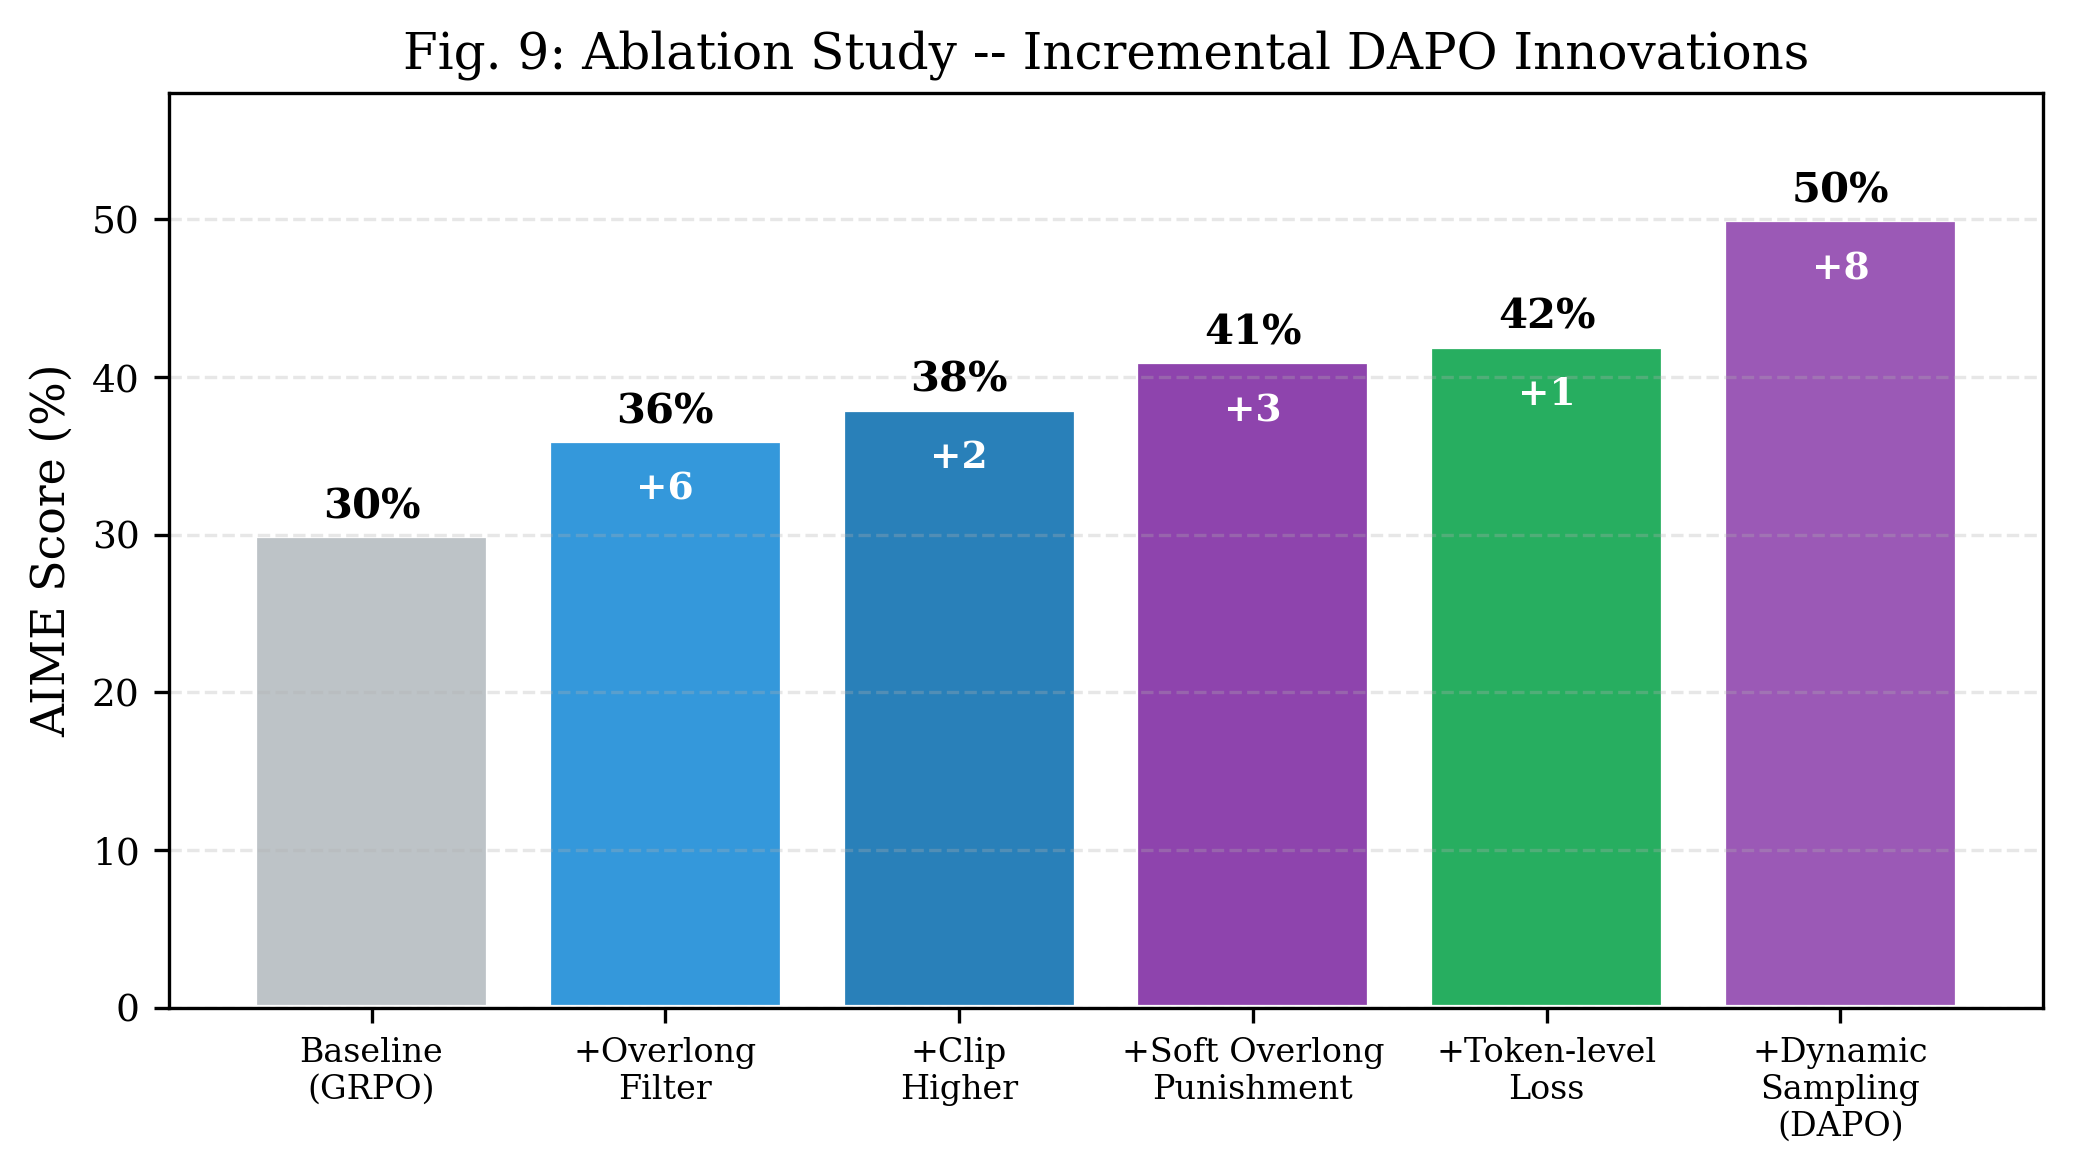
\includegraphics[width=\columnwidth]{ieee_fig9_ablation.png}
\caption{消融研究展示DAPO每项创新的增量贡献。动态采样提供最大单项提升（+8分），其次是过长过滤（+6分）。所有创新的组合效果使朴素GRPO提升20分。}
\label{fig:ablation}
\end{figure}

\textbf{消融实验的关键发现：}
\begin{enumerate}[leftmargin=*, itemsep=1pt]
\item \textbf{动态采样}贡献最大单项提升（+8分），通过确保每个批次包含信息性梯度。
\item \textbf{过长过滤}贡献第二大增益（+6分），移除了浪费容量的无信息长响应。
\item \textbf{Clip-Higher}添加+2分，在整个训练过程中维持探索能力。
\item \textbf{Token级损失}添加+1分，消除长度偏差，但单独效果相对温和。
\end{enumerate}

%=============================================================
\section{讨论与未来方向}
\label{sec:discuss}

\subsection{实用算法选择指南}

基于我们的分析，提供以下选择建议：

\begin{itemize}[leftmargin=*, itemsep=2pt]
\item \textbf{选择DPO}：当有高质量偏好数据时；任务涉及主观对齐（有用性、安全性）；优先考虑实现简洁性；GPU资源有限。
\item \textbf{选择GRPO}：当任务具有客观的规则型奖励时；内存效率至关重要；模型规模较小使熵坍塌不那么严重；需要快速原型开发。
\item \textbf{选择DAPO}：当需要最大推理性能时；涉及长链思维推理；有足够算力支持组采样；长时间训练的稳定性重要。
\item \textbf{选择PPO}：当需要学习型奖励模型时；任务涉及LLM对齐之外的通用RL；需要理论收敛保证；已有支持PPO的RLHF基础设施。
\end{itemize}

\subsection{开放性挑战}

\begin{enumerate}[leftmargin=*, itemsep=2pt]
\item \textbf{千亿参数规模的可扩展性：}四种算法在超大规模模型上都面临显著的工程挑战。组方法（GRPO、DAPO）每个提示词需要$G$次前向传播，对超大模型代价高昂。
\item \textbf{开放式任务的奖励规范：}数学推理受益于规则型奖励，但将这些方法扩展到创意写作、对话和开放生成仍具挑战性。
\item \textbf{长度利用：}模型可能学会利用基于长度的奖励信号（如生成不必要的长链思维推理）。DAPO的过长奖励整形部分解决了这一问题，但需要更鲁棒的解决方案。
\item \textbf{样本效率：}组方法每个提示词每步需要$G$个样本，比单样本方法代价高$G$倍。在保持优势质量的同时降低这一开销是重要的开放问题。
\item \textbf{多目标优化：}实际LLM部署需要同时平衡准确性、安全性、有用性和效率。当前算法优化单一标量奖励，可能无法最优地捕捉这些权衡。
\end{enumerate}

\subsection{有前景的研究方向}

\begin{enumerate}[leftmargin=*, itemsep=2pt]
\item \textbf{混合方法：}将DPO的离线偏好学习与DAPO的Token级在线优化相结合，发挥两种范式的优势。
\item \textbf{过程奖励模型（PRM）：}步骤级奖励信号~\cite{lightman2024verify, uesato2022solving, wang2024mathshepherd}可替代结果级奖励，为链思维推理提供更丰富的训练信号。
\item \textbf{自适应组采样：}根据提示词难度动态调整$G$，在保持优势质量的同时降低计算浪费。
\item \textbf{投机解码加速组采样：}使用投机解码更高效地生成组样本，可显著降低GRPO/DAPO的开销。
\item \textbf{元学习算法选择：}训练元学习器为给定任务选择最优RL算法和超参数，自动化算法选择过程。
\end{enumerate}

%=============================================================
\section{结论}
\label{sec:conclusion}

本综述对四种大语言模型训练中的强化学习算法——PPO、DPO、GRPO和DAPO——进行了全面系统的分析。我们的贡献包括统一数学框架（一致符号）、详细的架构比较以及数学推理基准上的实验评估。

分析揭示了该领域的清晰演进轨迹：
\begin{itemize}[leftmargin=*, itemsep=1pt]
\item \textbf{PPO}（2017年）建立了裁剪代理基础和双网络架构，支撑了第一代对齐LLM（InstructGPT、ChatGPT）。
\item \textbf{DPO}（2023年）证明了通过消除显式奖励建模可以大幅简化RLHF流程，以在线探索换取离线简洁性。
\item \textbf{GRPO}（2025年）通过组优势归一化消除了价值网络，内存减少$\sim$50\%，简化了可验证推理任务的架构。
\item \textbf{DAPO}（2025年）通过三项针对性创新扩展GRPO——非对称Clip-Higher、动态采样和Token级损失——在AIME 2024上实现67\%的相对提升。
\end{itemize}

对实践者的建议明确：对于有偏好数据的主观对齐任务使用\textbf{DPO}，对于资源受限的高效推理使用\textbf{GRPO}，对于追求最大推理性能使用\textbf{DAPO}，当需要学习型奖励模型和理论保证时使用\textbf{PPO}。该领域正在快速发展，混合方法和过程级反馈代表了特别有前景的未来研究方向。

%=============================================================
\section*{参考文献}
\begin{thebibliography}{30}

\bibitem{schulman2017ppo}
J.~Schulman, F.~Wolski, P.~Dhariwal, A.~Radford, and O.~Klimov, ``Proximal policy optimization algorithms,'' \textit{arXiv preprint arXiv:1707.06347}, 2017.

\bibitem{schulman2016gae}
J.~Schulman, P.~Moritz, S.~Levine, M.~Jordan, and P.~Abbeel, ``High-dimensional continuous control using generalized advantage estimation,'' in \textit{Proc.\ ICLR}, 2016.

\bibitem{rafailov2023dpo}
R.~Rafailov, A.~Sharma, E.~Mitchell, S.~Ermon, C.~D.~Manning, and C.~Finn, ``Direct preference optimization: Your language model is secretly a reward model,'' in \textit{Proc.\ NeurIPS}, 2023.

\bibitem{deepseek2025r1}
DeepSeek-AI, ``DeepSeek-R1: Incentivizing reasoning capability in LLMs via reinforcement learning,'' \textit{arXiv preprint arXiv:2501.12948}, 2025.

\bibitem{yu2025dapo}
Q.~Yu \textit{et al.}, ``DAPO: An open-source LLM reinforcement learning system at scale,'' \textit{arXiv preprint arXiv:2503.14476}, 2025.

\bibitem{ouyang2022instructgpt}
L.~Ouyang \textit{et al.}, ``Training language models to follow instructions with human feedback,'' in \textit{Proc.\ NeurIPS}, 2022.

\bibitem{christo2017deep}
P.~F.~Christiano \textit{et al.}, ``Deep reinforcement learning from human preferences,'' in \textit{Proc.\ NeurIPS}, 2017.

\bibitem{ziegler2019fine}
D.~M.~Ziegler \textit{et al.}, ``Fine-tuning language models from human preferences,'' \textit{arXiv preprint arXiv:1909.08593}, 2019.

\bibitem{stiennon2020learning}
N.~Stiennon \textit{et al.}, ``Learning to summarize with human feedback,'' in \textit{Proc.\ NeurIPS}, 2020.

\bibitem{bai2022training}
Y.~Bai \textit{et al.}, ``Training a helpful and harmless assistant with reinforcement learning from human feedback,'' \textit{arXiv preprint arXiv:2204.05862}, 2022.

\bibitem{touvron2023llama}
H.~Touvron \textit{et al.}, ``LLaMA: Open and efficient foundation language models,'' \textit{arXiv preprint arXiv:2302.13971}, 2023.

\bibitem{achiam2023gpt4}
J.~Achiam \textit{et al.}, ``GPT-4 technical report,'' \textit{arXiv preprint arXiv:2303.08774}, 2023.

\bibitem{zheng2023secrets}
L.~Zheng \textit{et al.}, ``Secrets of RLHF in large language models part I: PPO,'' \textit{arXiv preprint arXiv:2307.04964}, 2023.

\bibitem{yuan2024self}
W.~Yuan \textit{et al.}, ``Self-rewarding language models,'' \textit{arXiv preprint arXiv:2401.10020}, 2024.

\bibitem{cui2024ultrafeedback}
G.~Cui \textit{et al.}, ``UltraFeedback: Boosting language models with scaled AI feedback,'' \textit{arXiv preprint arXiv:2310.01377}, 2024.

\bibitem{wang2024helpsteer}
Z.~Wang \textit{et al.}, ``HelpSteer: Multi-attribute helpfulness dataset for SteerLM,'' \textit{arXiv preprint arXiv:2311.09528}, 2024.

\bibitem{meng2024simpo}
Y.~Meng \textit{et al.}, ``SimPO: Simple preference optimization with reference-free reward,'' \textit{arXiv preprint arXiv:2405.14734}, 2024.

\bibitem{hong2024orpo}
J.~Hong \textit{et al.}, ``ORPO: Monolithic preference optimization without reference model,'' \textit{arXiv preprint arXiv:2403.07691}, 2024.

\bibitem{azar2024general}
M.~G.~Azar \textit{et al.}, ``A general theoretical paradigm to understand learning from human preferences,'' in \textit{Proc.\ ICML}, 2024.

\bibitem{rosset2024direct}
C.~Rosset \textit{et al.}, ``Direct Nash optimization: Teaching language models to self-improve more effectively,'' \textit{arXiv preprint arXiv:2404.03715}, 2024.

\bibitem{shao2024deepseekmath}
Z.~Guo \textit{et al.}, ``DeepSeekMath: Pushing the limits of mathematical reasoning in open language models,'' \textit{arXiv preprint arXiv:2402.03300}, 2024.

\bibitem{qwen2024qwen2}
Qwen Team, ``Qwen2 technical report,'' \textit{arXiv preprint arXiv:2407.10671}, 2024.

\bibitem{yang2024qwen25}
A.~Yang \textit{et al.}, ``Qwen2.5 technical report,'' \textit{arXiv preprint arXiv:2412.15115}, 2024.

\bibitem{dubey2024llama3}
A.~Dubey \textit{et al.}, ``The Llama 3 herd of models,'' \textit{arXiv preprint arXiv:2407.21783}, 2024.

\bibitem{snell2024scaling}
C.~Snell \textit{et al.}, ``Scaling LLM test-time compute optimally can be more effective than scaling model parameters,'' \textit{arXiv preprint arXiv:2408.03314}, 2024.

\bibitem{lightman2024verify}
H.~Lightman \textit{et al.}, ``Let's verify step by step,'' in \textit{Proc.\ ICLR}, 2024.

\bibitem{uesato2022solving}
J.~Uesato \textit{et al.}, ``Solving math word problems with process and outcome-based feedback,'' in \textit{Proc.\ NeurIPS}, 2022.

\bibitem{wang2024mathshepherd}
P.~Wang \textit{et al.}, ``Math-Shepherd: Verify and reinforce LLMs step-by-step,'' \textit{arXiv preprint arXiv:2312.08935}, 2024.

\bibitem{zeng2024glm4}
A.~Zeng \textit{et al.}, ``GLM-4 technical report,'' \textit{arXiv preprint arXiv:2406.12793}, 2024.

\end{thebibliography}


\end{document}
